\documentclass[a4paper,12pt]{article}
\usepackage[a4paper,top=1.3cm,bottom=2cm,left=1.5cm,right=1.5cm,marginparwidth=0.75cm]{geometry}
\usepackage{cmap}
\usepackage{mathtext}
\usepackage[T2A]{fontenc}
\usepackage[utf8]{inputenc}
\usepackage[english,russian]{babel}
\usepackage{siunitx}
\usepackage{enumitem}
\usepackage{placeins}

\usepackage{graphicx}
\usepackage{subcaption}
\usepackage{amsmath}

\usepackage{wrapfig}
\usepackage{tabularx}
\usepackage{multirow}

\usepackage{hyperref}
\usepackage[rgb]{xcolor}
\hypersetup{colorlinks=true,urlcolor=blue}
\usepackage{siunitx}
\usepackage{amsmath,amsfonts,amssymb,amsthm,mathtools}
\usepackage{mathtools}
\usepackage{icomma}
\mathtoolsset{showonlyrefs=false}
\usepackage{euscript}
\usepackage{mathrsfs}
\DeclareMathOperator{\sgn}{\mathop{sgn}}
\newcommand*{\hm}[1]{#1\nobreak\discretionary{}
{\hbox{$\mathsurround=0pt #1$}}{}}

\newcommand\labname{Применения операционных усилителей}
\newcommand\labnumber{77}

\author{Макаров Лев Евгеньевич}
\title{Лабораторная работа №\labnumber\\\labname}
\date{\today}

\makeatletter
\AddEnumerateCounter{\asbuk}{\russian@asbuk@alph}{щ}
\makeatother
\begin{document}

\begin{titlepage}
    \begin{center}
        {\large МОСКОВСКИЙ ФИЗИКО-ТЕХНИЧЕСКИЙ ИНСТИТУТ (НАЦИОНАЛЬНЫЙ ИССЛЕДОВАТЕЛЬСКИЙ УНИВЕРСИТЕТ)}
    \end{center}
    \begin{center}
        {\large Физтех-школа фотоники, электроники и молекулярной физики}
    \end{center}

    \vspace{4.5cm}
    {\huge
        \begin{center}
            {\bf Отчёт о выполнении лабораторной работы \labnumber}\\
            \labname
        \end{center}
    }
    \vspace{2cm}
    \begin{flushright}
        {\LARGE Автор:\\ Макаров Лев Евгеньевич\\
        \vspace{0.2cm}
        Б04-306}
    \end{flushright}
    \vspace{8cm}
    \begin{center}
        Долгопрудный 2026
    \end{center}
\end{titlepage}

\section{Введение}


\textbf{Цель работы:} Исследовать способы применения операционных усилителей

\section{Выполнение работы}

\subsection*{Измерение коэффициента усиления ОУ}

\begin{enumerate}
    \item Соберем схему согласно рис. \ref{pic:ustan-1}. Измеренные сопротивления резисторов в схеме представлены в таблице \ref{tab:params-1}.
\end{enumerate}

\FloatBarrier
\begin{table}[!h]
    \centering
    \caption{Измеренные параметры установки в схеме на рис. \ref{pic:ustan-1}}
    \label{tab:params-1}
    \begin{tabular}{|l|l|l|l|}
        \hline
        $R_1$, кОм & $R_2$, кОм & $R_3$, кОм & $R_4$, кОм \\ \hline
        107.2      & 107.1      & 107.8      & 1.08       \\ \hline
    \end{tabular}
\end{table}


\begin{figure}[h]
    \centering
    
\includegraphics[width=0.35\textwidth]{pictures/ustan-1.png}
    \caption{Схема измерения коэффициента усиления}
    \label{pic:ustan-1}
\end{figure}
\FloatBarrier

\begin{enumerate}[resume]
    \item Подадим на вход колебания с амплитудой $U_\textit{in} = 2.5~\text{В}$ и частотой $f = 10~\text{Гц}$. Тогда измеренные напряжения
\end{enumerate}

\begin{equation*}
    U_a = 3.8~\text{мВ}; \qquad U_\textit{out} = 2.498~\text{В}
\end{equation*}

\begin{enumerate}[resume]
    \item Рассчитаем коэффициент усиления операционного усилителя по формуле:
\end{enumerate}

\begin{equation*}
    A_0 = \left( 1 + \cfrac{R_3}{R_4} \right) \cdot \cfrac{U_\textit{out}}{U_a} = 66272
\end{equation*}

\subsection*{Амплитудно-частотная характеристика ОУ}

\begin{enumerate}
    \item Для схемы на рис. \ref{pic:ustan-1} снимем зависимость коэффициента усиления от частоты. Результаты измерений представлены в таблице \ref{tab:data-2}.
\end{enumerate}

\begin{table}[!h]
    \centering
    \caption{Измерение АЧХ операционного усилителя}
    \label{tab:data-2}
    \begin{tabular}{l|l|l|l}
        \hline
        $U_a$, мВ & $U_\textit{out}$, В & $A$ & $f$, Гц \\ \hline
        8.6  & 2.54   & 29775 & 50      \\
        16.5 & 2.545  & 15456 & 100     \\
        35   & 2.549  & 7342  & 200     \\ 
        89.5 & 2.535  & 2855  & 500     \\ 
        176  & 2.49   & 1426  & 1000    \\ 
        321  & 2.3    & 722   & 2000    \\ 
        590  & 1.725  & 294   & 5000    \\ 
        742  & 1.055  & 143   & 10000   \\ 
        780  & 0.545  & 70    & 20000   \\ 
        795  & 0.222  & 28    & 50000   \\ 
        740  & 0.1    & 13    & 100000  \\ 
        540  & 0.037  & 6.9   & 200000  \\ 
        355  & 0.0085 & 2.4   & 500000  \\ 
        202  & 1.94   & 0.96  & 1000000 \\ \hline
    \end{tabular}
\end{table}


\begin{enumerate}[resume]
    \item Построим снятую зависимость в двойном логарифмическом масштабе, откладывая коэффициент усиления в децибелах, а частоту в герцах. Изобразим график на рис. \ref{pic:graph_achx}
\end{enumerate}

\begin{figure}[h]
    \centering
    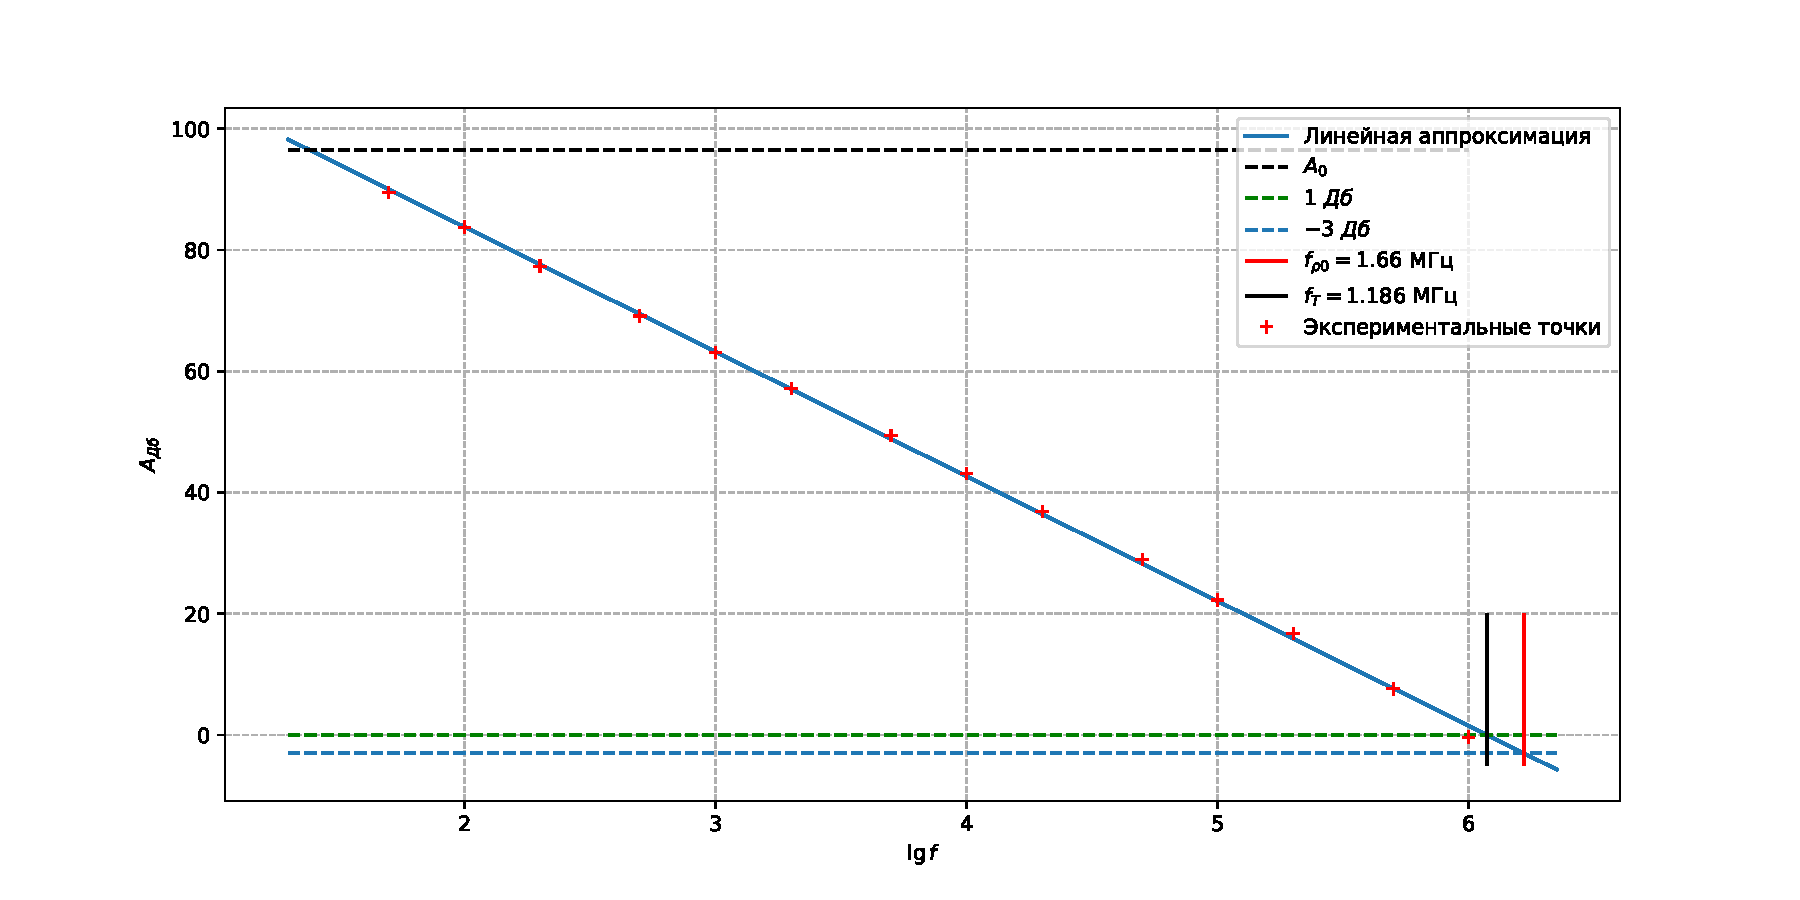
\includegraphics[width=\textwidth]{pictures/graph_achx.pdf}
    \caption{Зависимость $A_\text{Дб}$ от $\lg{f}$ для операционного усилителя}
    \label{pic:graph_achx}
\end{figure}

\clearpage

\subsection*{Неинвертирующий усилитель}

\begin{figure}[h]
    \centering
    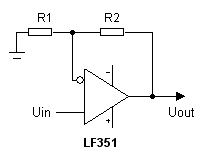
\includegraphics[width=0.35\textwidth]{pictures/ustan-3.png}
    \caption{Схема неинвертирующего усилителя}
    \label{pic:ustan-3}
\end{figure}

\begin{enumerate}
    \item Соберем схему, изображенную на рис. \ref{pic:ustan-3} так, чтобы $R_2 / R_1 \sim 100 - 200$. 
\end{enumerate}

\begin{table}[!h]
    \centering
    \caption{Измеренные параметры установки в схеме на рис. \ref{pic:ustan-3}}
    \label{tab:params-3}
    \begin{tabular}{|l|l|l|l|}
        \hline
        $R_1$, кОм & $R_2$, кОм \\ \hline
        1.08       & 107.8      \\ \hline
    \end{tabular}
\end{table}

\begin{enumerate}[resume]
    \item Измерим постоянное напряжение на выходе $U_\textit{out(dc)} = 50~\text{мВ}$. Рассчитаем входное напряжение сдвига:
\end{enumerate}

\begin{equation*}
    U_\textit{OS} = \cfrac{U_\textit{out(dc)}}{1 + \cfrac{R_2}{R_1}} = 0.5~\text{мВ}
\end{equation*}

\begin{enumerate}[resume]
    \item Снимем зависимость коэффициента усиления от частоты $K(f)$. Данные представлены в таблице \ref{tab:data-3}. Амплитуда входного сигнала $\widehat{U} = 51$ мВ. Изобразим график зависимости на рис. \ref{pic:graph_K_f}.
\end{enumerate}

\begin{table}[!h]
    \centering
    \caption{Измерение зависимости $K(f)$}
    \label{tab:data-3}
    \begin{tabular}{l|l|l}
        \hline
        $U_\textit{out}$, В & $f$, кГц & $K$ \\ \hline
        5    & 1    & 98  \\
        5.27 & 2    & 103 \\
        5.21 & 3    & 102 \\
        5.12 & 4    & 100 \\
        5.01 & 5    & 98  \\
        4.89 & 6    & 96  \\
        4.75 & 7    & 93  \\
        4.61 & 8    & 90  \\
        4.47 & 9    & 88  \\
        4.33 & 10   & 85  \\
        4.18 & 11   & 82  \\
        4.04 & 12   & 79  \\
        3.89 & 13   & 76  \\
        3.75 & 14   & 74  \\
        3.62 & 15   & 71  \\
        3.5  & 16   & 69  \\
        3.68 & 14.5 & 72  \\
        5.32 & 0.9  & 104 \\
        5.32 & 0.8  & 104 \\
        5.33 & 0.1  & 105 \\
        5.22 & 0.01 & 102 \\ \hline
    \end{tabular}
\end{table}

\begin{figure}[h]
    \centering
    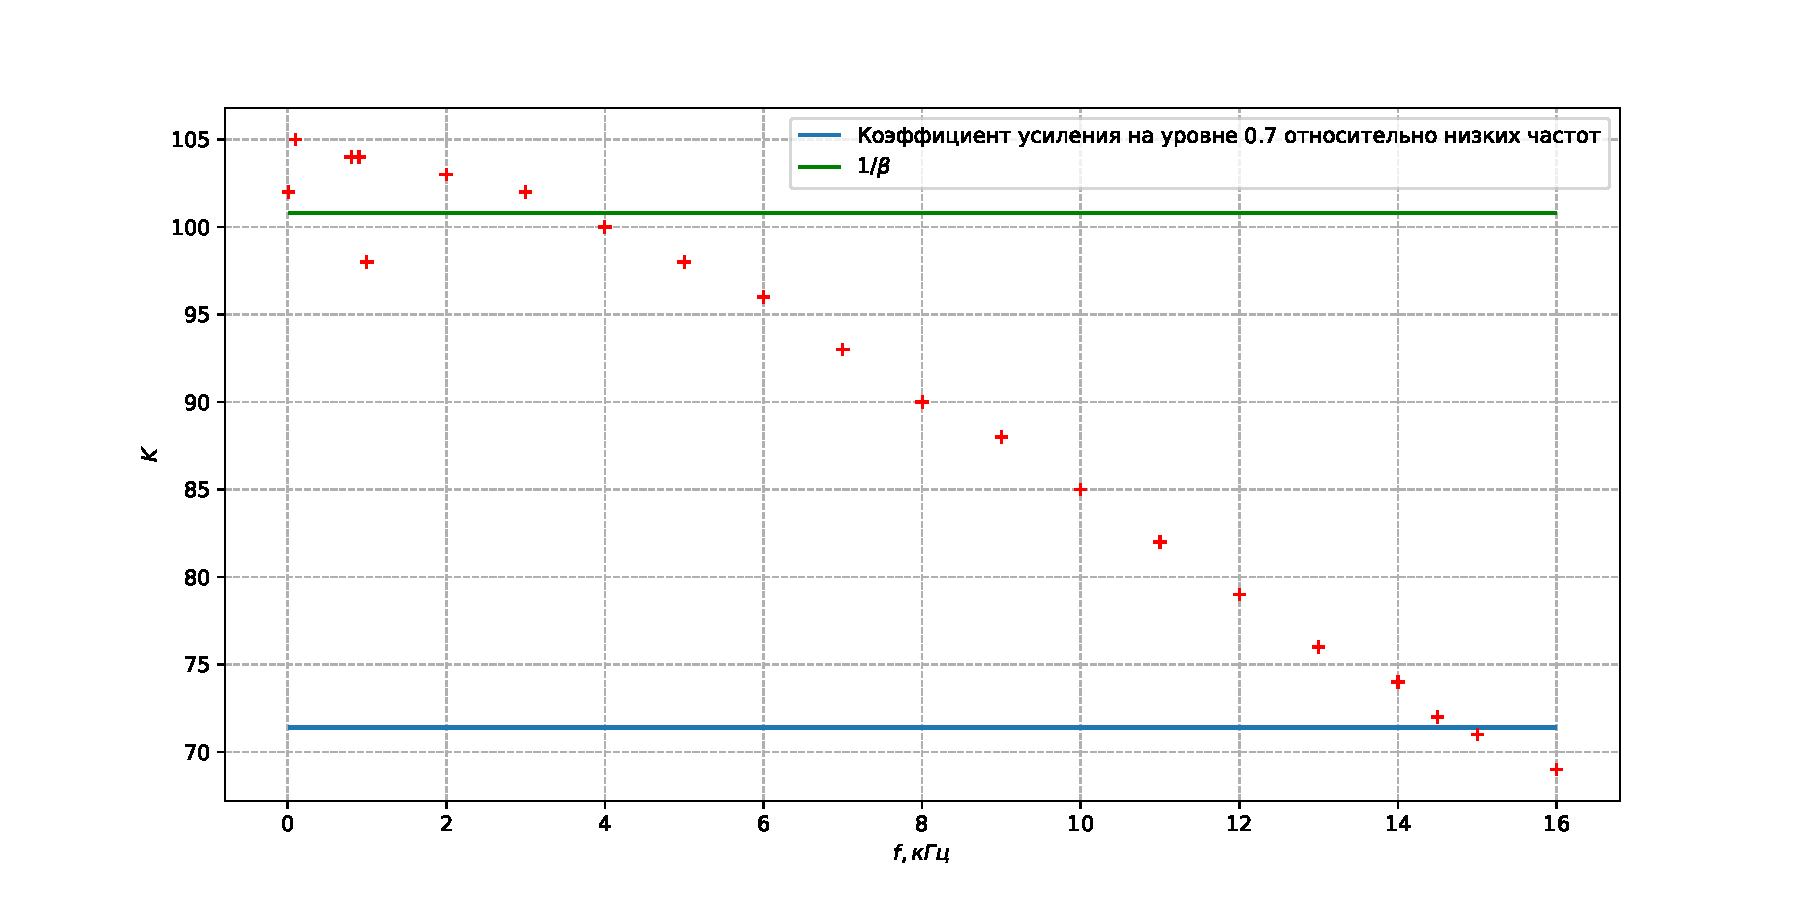
\includegraphics[width=\textwidth]{pictures/graph_K_f.pdf}
    \caption{Зависимость $K$ от $f$}
    \label{pic:graph_K_f}
\end{figure}

По графику можно определить граничную частоту $F_p = 14.75$ кГц.

\begin{enumerate}[resume]
    \item Проверим некоторые соотношения для коэффициента усиления.
\end{enumerate}

Коэффициент отрицательной обратной связи

\begin{equation*}
    \beta = \cfrac{R_1}{R_1 + R_2} = 9.92 \cdot 10^{-3}
\end{equation*}

Проверим $K_0 = 1 / \beta$

\begin{equation*}
    \cfrac{1}{\beta} = \cfrac{1}{9.92 \cdot 10^{-3}} = 100.8 \approx K_0
\end{equation*}

Для наглядности изобразим $1 / \beta$ на рис. \ref{pic:graph_K_f}.

Так же проверим $F_p = \beta f_T$

\begin{equation*}
    \beta f_T = 9.92 \cdot 10^{-3} \cdot 1.186 \cdot 10^6 = 11.7 ~\text{кГц}
\end{equation*}

Как видно соотношения приблизительно выполняется Но при этом $F_p = \beta f_T$ выполняется заметно хуже.

\clearpage
\begin{enumerate}[resume]
    \item Определим максимальную амплитуду неискаженного выходного сигнала
\end{enumerate}

\begin{equation*}
    U_\textit{in}^\textit{max} = 0.1749 ~ \text{В}; \qquad U_\textit{out}^\textit{max} = 17.9 ~ \text{В}
\end{equation*}

\begin{enumerate}[resume]
    \item Включим ОУ по схеме повторителя ($R_1 = \infty$ - разомкнуть, $R_2 = 0$ - закоротить). Измерим коэффициент передачи и граничную частоту усилителя. На частоте $f = 0.5$ МГц определим максимальную амплитуду неискаженного сигнала:
\end{enumerate}

\begin{equation*}
    U_\textit{in}^\textit{max} = 2.15 ~ \text{В}; \qquad U_\textit{out}^\textit{max} = 2.17 ~ \text{В}
\end{equation*}

При расчете по формуле:

\begin{equation*}
    U_\textit{out}^\textit{max} = \cfrac{V_\textit{max}}{2 \pi f} = \cfrac{3}{2 \cdot 3.14 \cdot 0.5} \approx 0.95 ~ \text{В}
\end{equation*}

Так как был измерен размах, а по формуле амплитуда, то различия в два раза означают, что теория примерно сходится с экспериментом.

\subsection*{Интегратор}

\begin{figure}[h]
    \centering
    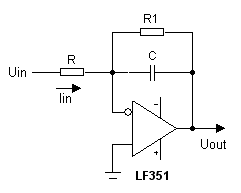
\includegraphics[width=0.35\textwidth]{pictures/ustan-8.png}
    \caption{Схема интегратора}
    \label{pic:ustan-8}
\end{figure}

\begin{enumerate}
    \item Рассчитаем элементы для схемы на рис. \ref{pic:ustan-8}.
\end{enumerate}

\begin{equation*}
    RC = 0.7 ~ \text{мс} \qquad \cfrac{R_1}{R} = 10
\end{equation*}

Выберем $C = 1.05$ мкФ, тогда $R = 700$ Ом, соответственно $R_1 = 7$ кОм. Измеренные значения выбранных компонентов представлены в таблице \ref{tab:params-8}.

\begin{table}[!h]
    \centering
    \caption{Измеренные параметры установки в схеме на рис. \ref{pic:ustan-8}}
    \label{tab:params-8}
    \begin{tabular}{|l|l|l|}
        \hline
        $R$, Ом & $R_1$, кОм & $C$, мкФ \\ \hline
        668     & 6.72       & 1.05     \\ \hline
    \end{tabular}
\end{table}

\begin{enumerate}[resume]
    \item Снимем АЧХ интегратора, изобразим ее на рис. \ref{pic:graph_achx_8}. Данные представлены в таблице \ref{tab:data-8}.
\end{enumerate}

\begin{table}[h]
    \centering
    \caption{Измерение АЧХ интегратора}
    \begin{minipage}[t]{0.48\textwidth}
        \centering
        \begin{tabular}{l|l|l|l}
            \hline
            $\hat{a}$, мВ & $A_\textit{out}$, мВ & $f$, Гц & $K$ \\ \hline
            444 & 3760 & 5    & 8.47 \\
            444 & 3760 & 10   & 8.47 \\
            444 & 3526 & 15   & 7.94 \\
            444 & 3222 & 20   & 7.26 \\
            444 & 3100 & 22   & 6.98 \\
            300 & 1300 & 50   & 4.33 \\
            300 & 503  & 150  & 1.68 \\
            300 & 306  & 250  & 1.02 \\
            300 & 224  & 350  & 0.75 \\
            300 & 174  & 450  & 0.58 \\
            300 & 143  & 550  & 0.48 \\
            300 & 120  & 650  & 0.40 \\
            300 & 104  & 750  & 0.35 \\
            300 & 92   & 850  & 0.31 \\
            300 & 82   & 950  & 0.27 \\
            300 & 74   & 1050 & 0.25 \\ \hline
        \end{tabular}
    \end{minipage}
    \hfill
    \begin{minipage}[t]{0.48\textwidth}
        \centering
        \begin{tabular}{l|l|l|l}
            \hline
            $\hat{a}$, мВ & $A_\textit{out}$, мВ & $f$, Гц & $K$ \\ \hline
            300 & 68   & 1150 & 0.23 \\
            300 & 62   & 1250 & 0.21 \\
            300 & 58   & 1350 & 0.19 \\
            300 & 54   & 1450 & 0.18 \\
            300 & 50   & 1550 & 0.17 \\
            300 & 47   & 1650 & 0.16 \\
            300 & 44   & 1750 & 0.15 \\
            300 & 42   & 1850 & 0.14 \\
            300 & 40   & 1950 & 0.13 \\
            300 & 38   & 2050 & 0.13 \\
            300 & 36   & 2150 & 0.12 \\
            300 & 24   & 2250 & 0.08 \\
            300 & 32   & 2350 & 0.11 \\
            300 & 31   & 2450 & 0.10 \\
            300 & 30   & 2550 & 0.10 \\
            300 & 29   & 2650 & 0.10 \\ \hline
        \end{tabular}
    \end{minipage}
\end{table}

\begin{figure}[h]
    \centering
    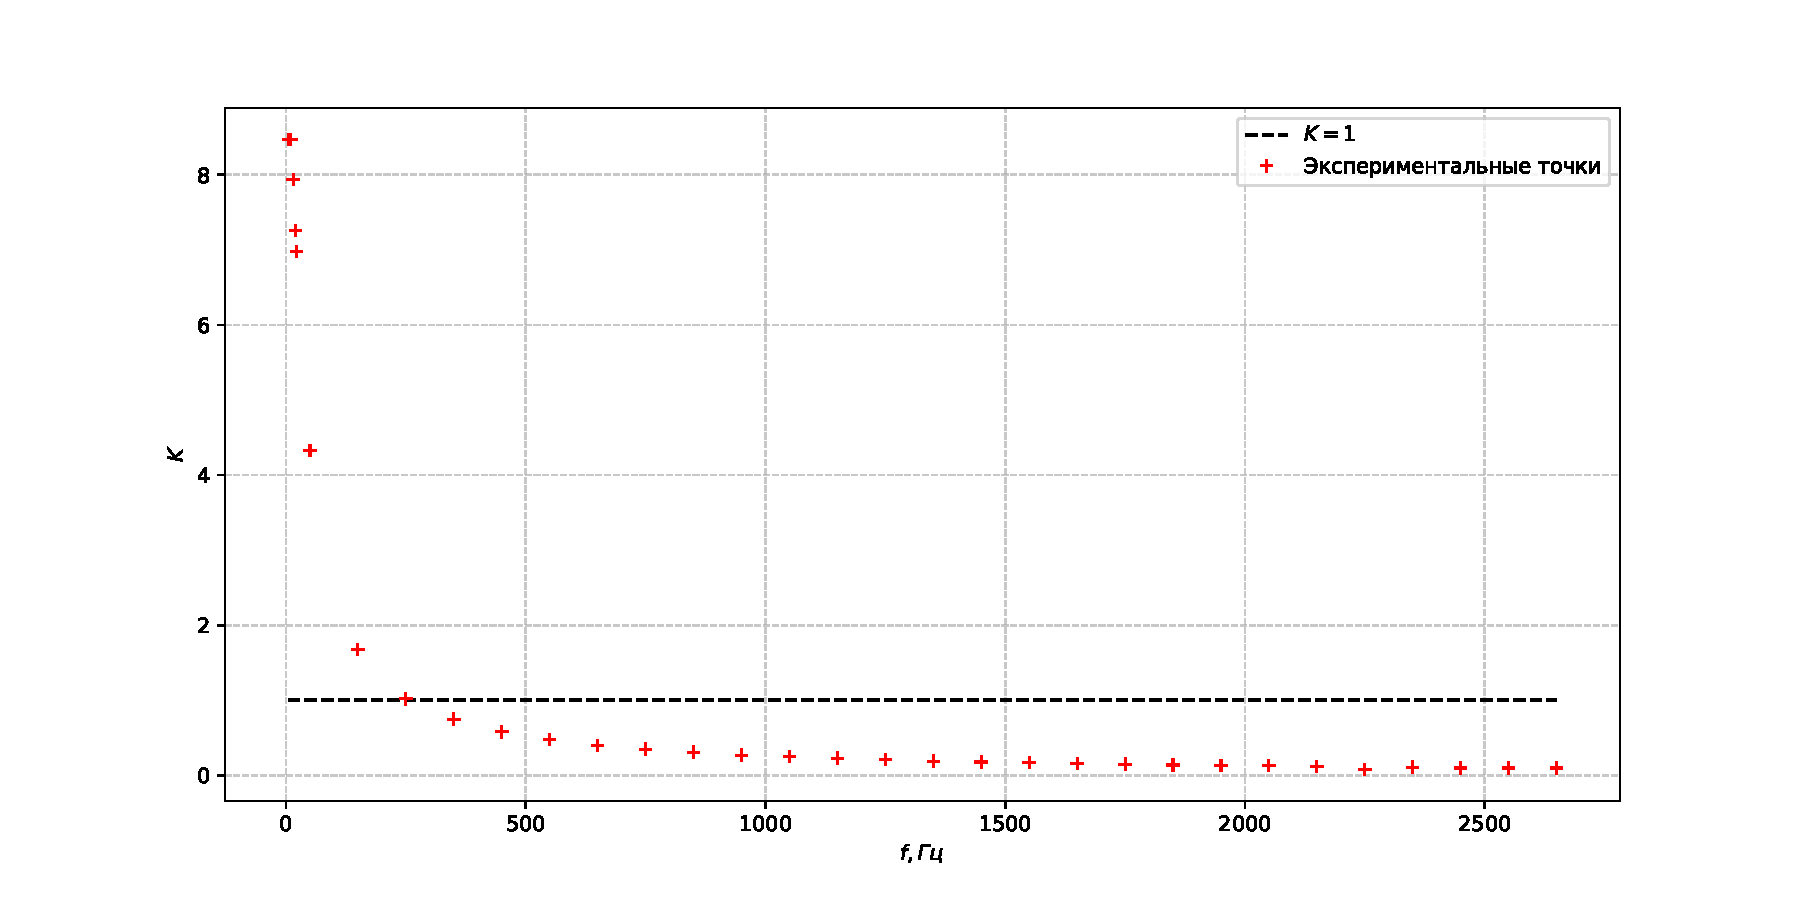
\includegraphics[width=\textwidth]{pictures/graph_achx_8.pdf}
    \caption{АЧХ интегратора}
    \label{pic:graph_achx_8}
\end{figure}
\FloatBarrier

По графику найдем частоту единичного усиления $F_1 = 250$ Гц.

Граничная частота:

\begin{equation*}
    f_0 = \cfrac{1}{2 \pi R_1 C} \approx 22 ~ \text{Гц}
\end{equation*}

Построим диаграмму Боде, изобразим ее на рис. \ref{pic:graph_bodee}

\FloatBarrier
\begin{figure}[h]
    \centering
    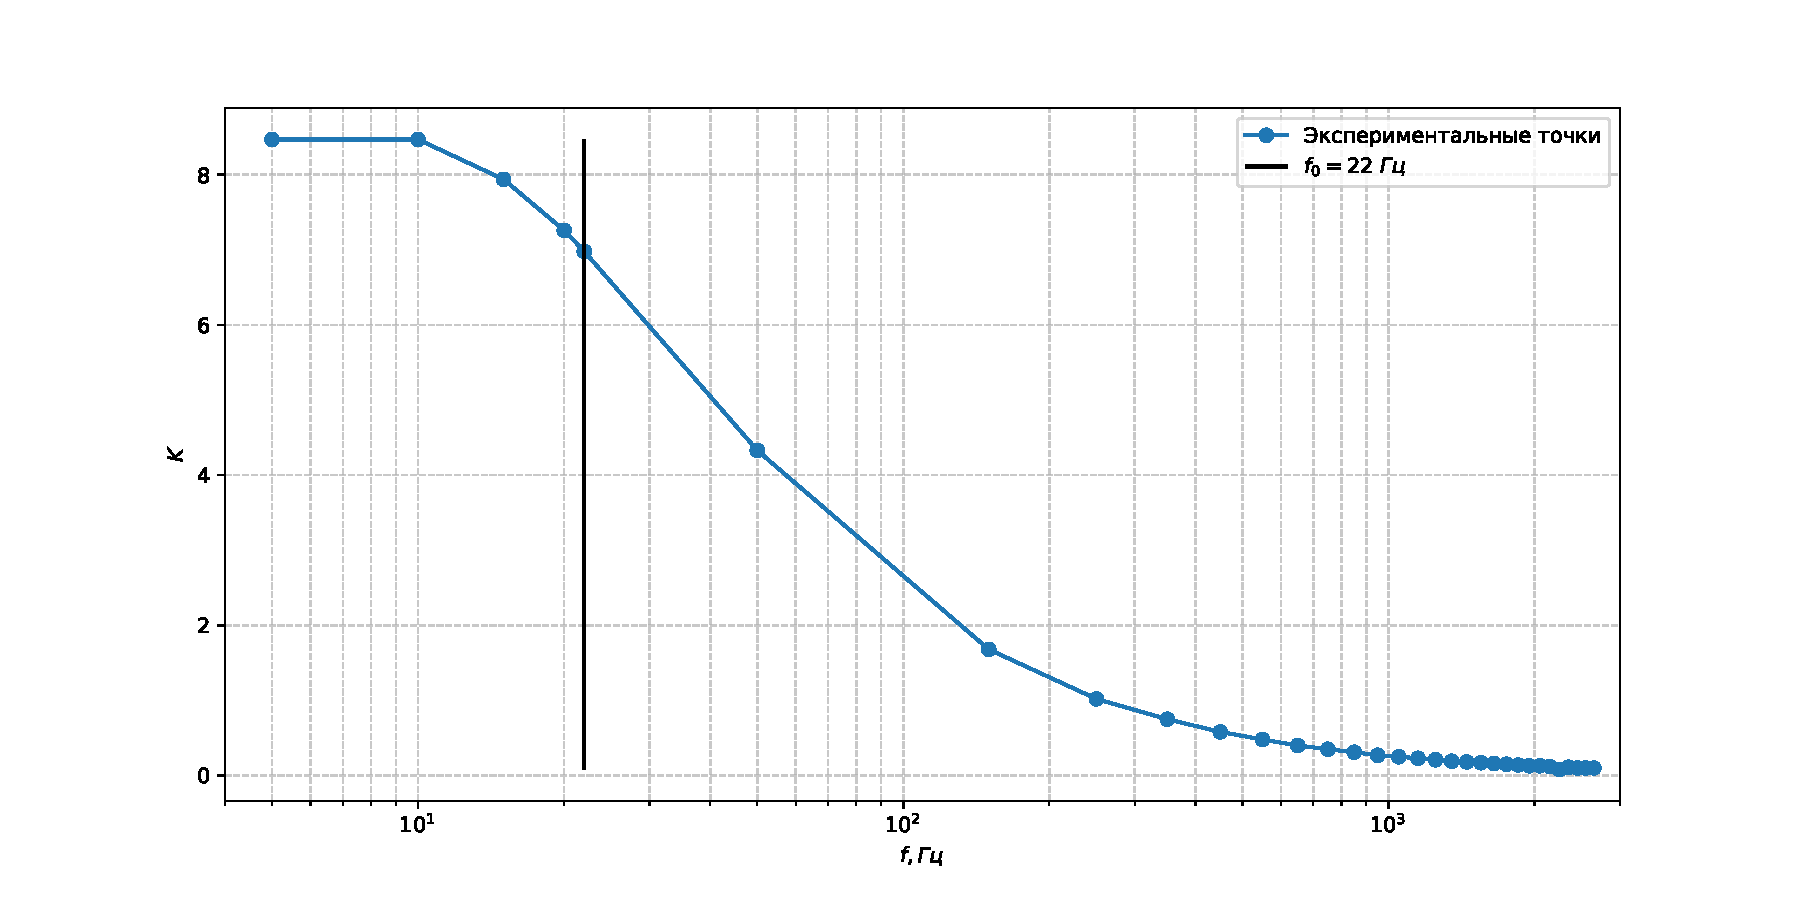
\includegraphics[width=\textwidth]{pictures/graph_bodee.pdf}
    \caption{Диаграмма Боде для интегратора}
    \label{pic:graph_bodee}
\end{figure}
\FloatBarrier

Как видно ниже частоты $f_0$ интегратор является усилителем. Тогда он является интегратором при частотах выше $f_0$.

\begin{enumerate}[resume]
    \item Подадим на вход интегратора треугольный и прямоугольный сигналы с амплитудой $\hat{a} = 1.6296$ В и частотой $f = 100$ Гц. Осциллограммы представлены на рис. \ref{pic:osc_triangle} и \ref{pic:osc_rectangle}. Синий цвет соответствует входному сигналу, зеленый - сигналу на выходе.
\end{enumerate}

\begin{figure}[h]
    \centering
    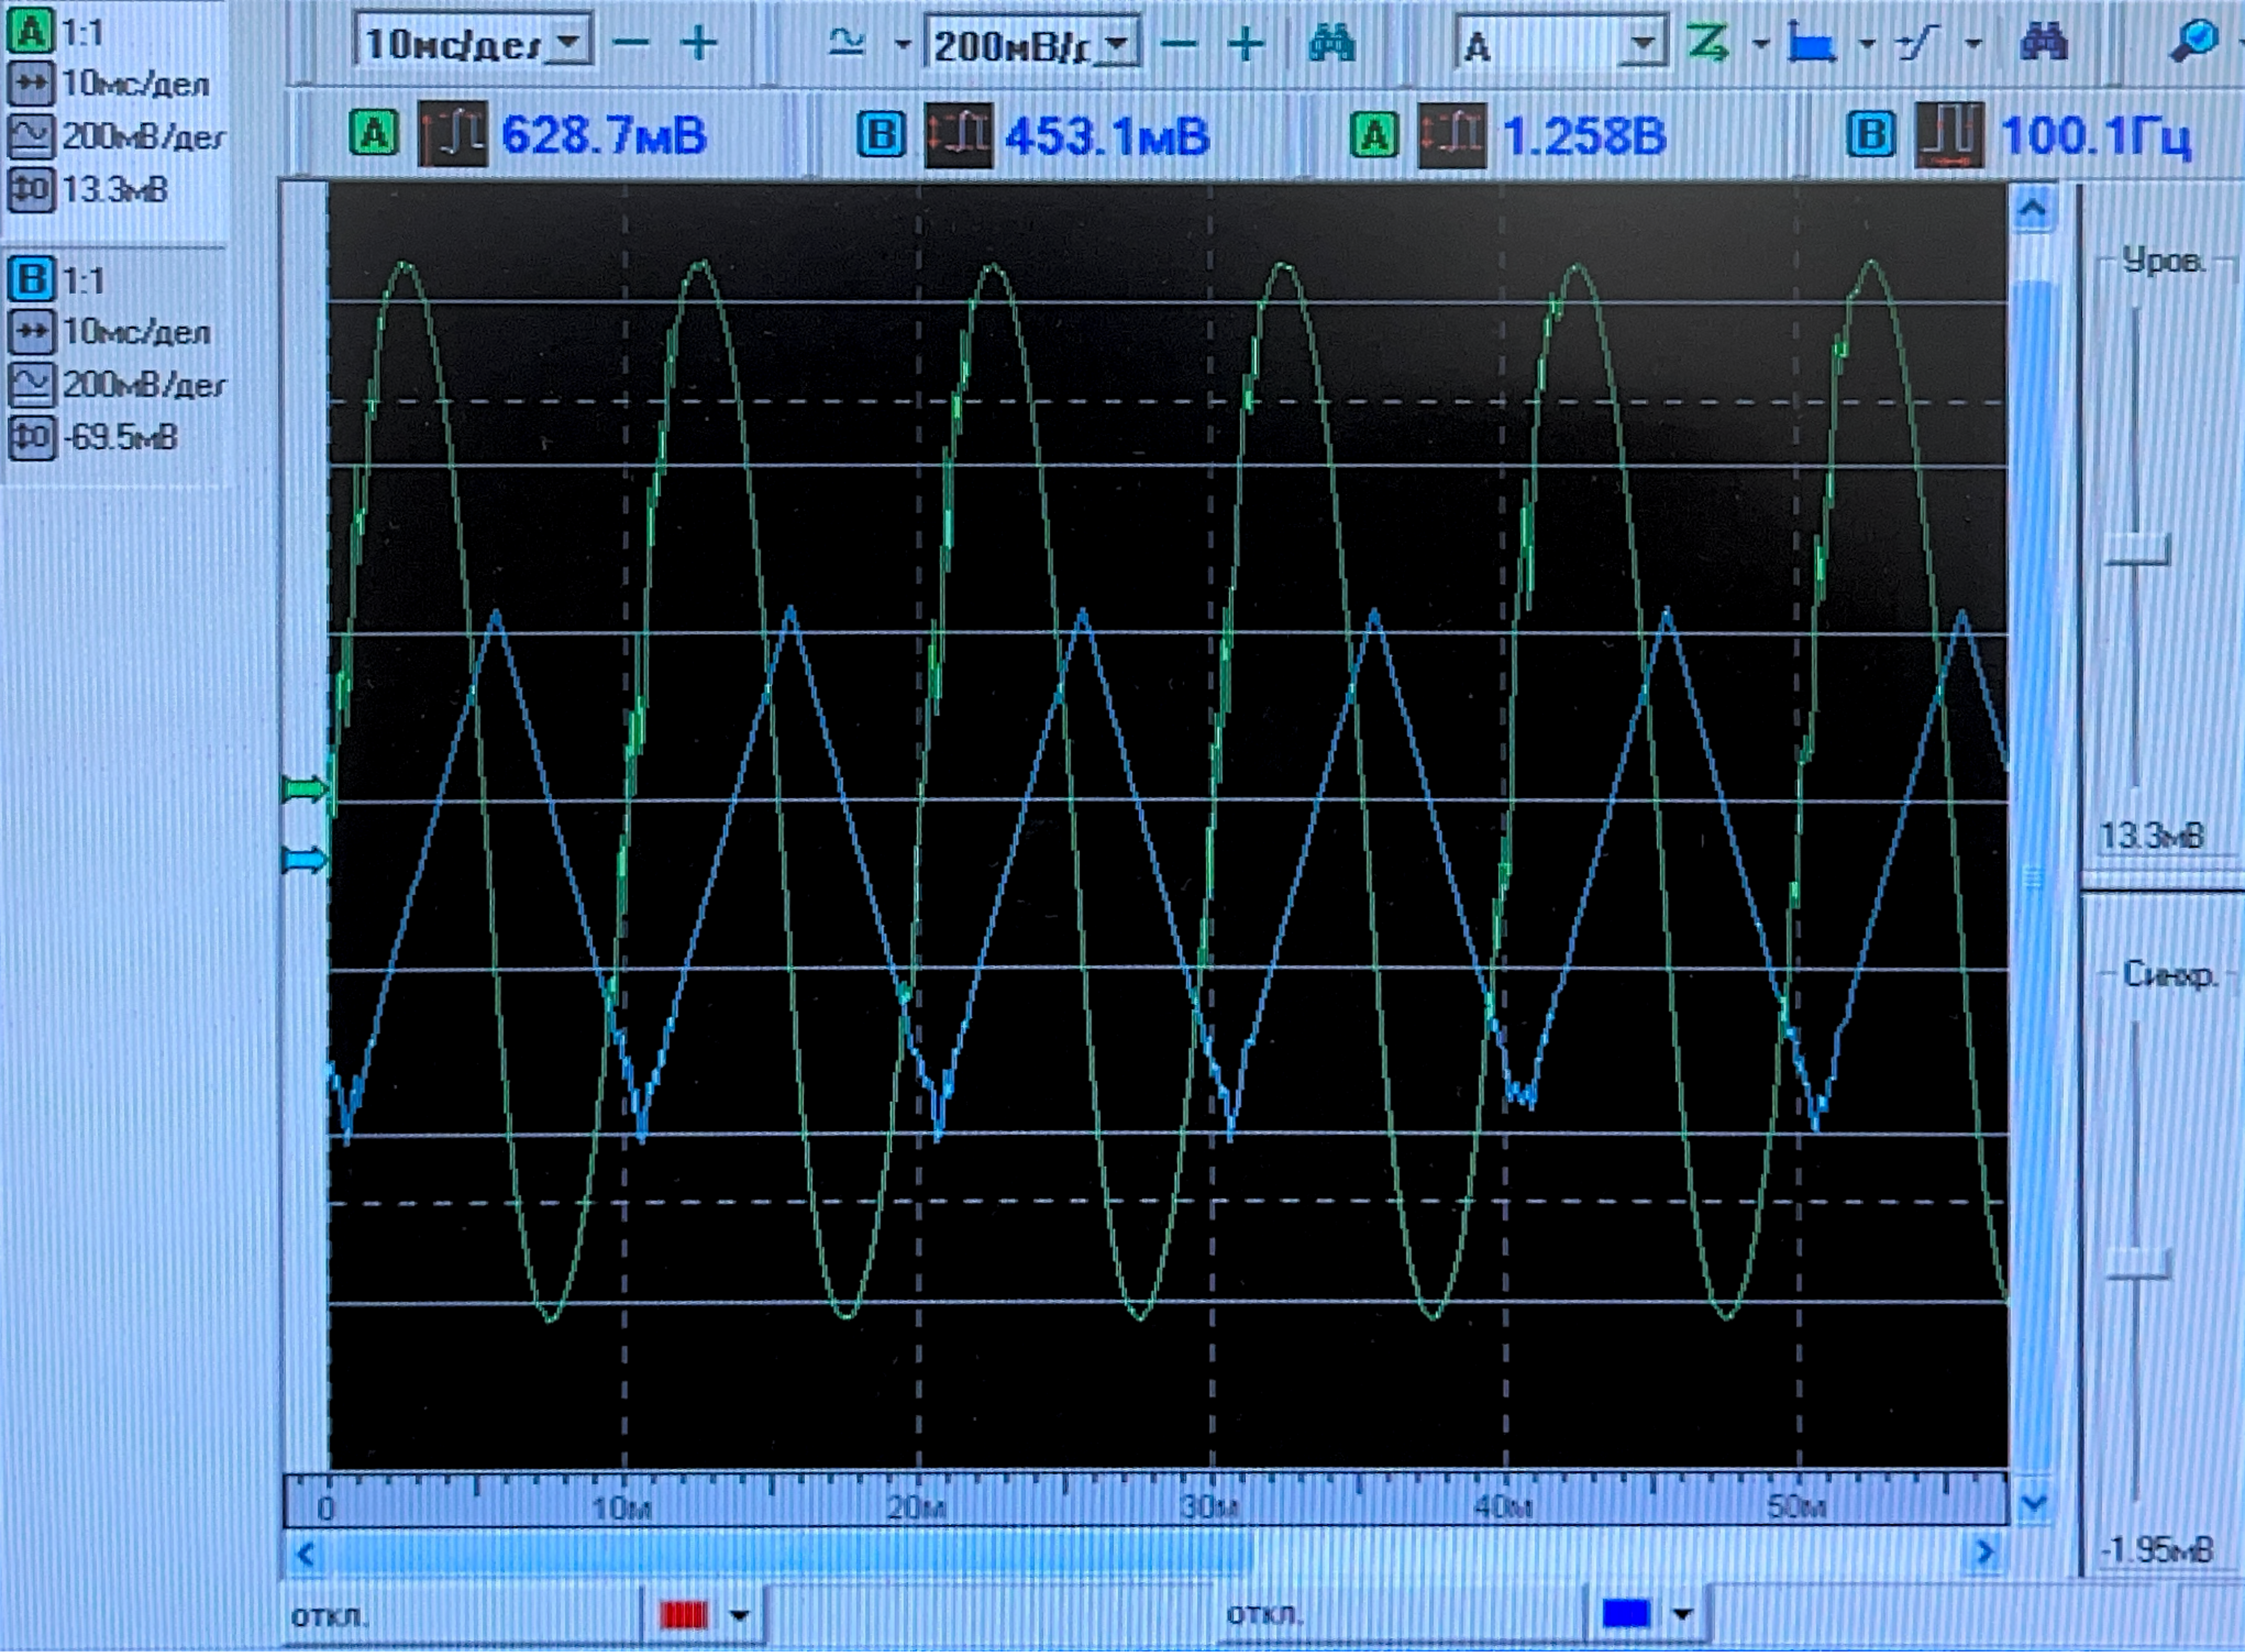
\includegraphics[width=0.7\textwidth]{pictures/osc_triangle.pdf}
    \caption{Осциллограмма для треугольного сигнала на входе интегратора}
    \label{pic:osc_triangle}
\end{figure}

\begin{figure}[h]
    \centering
    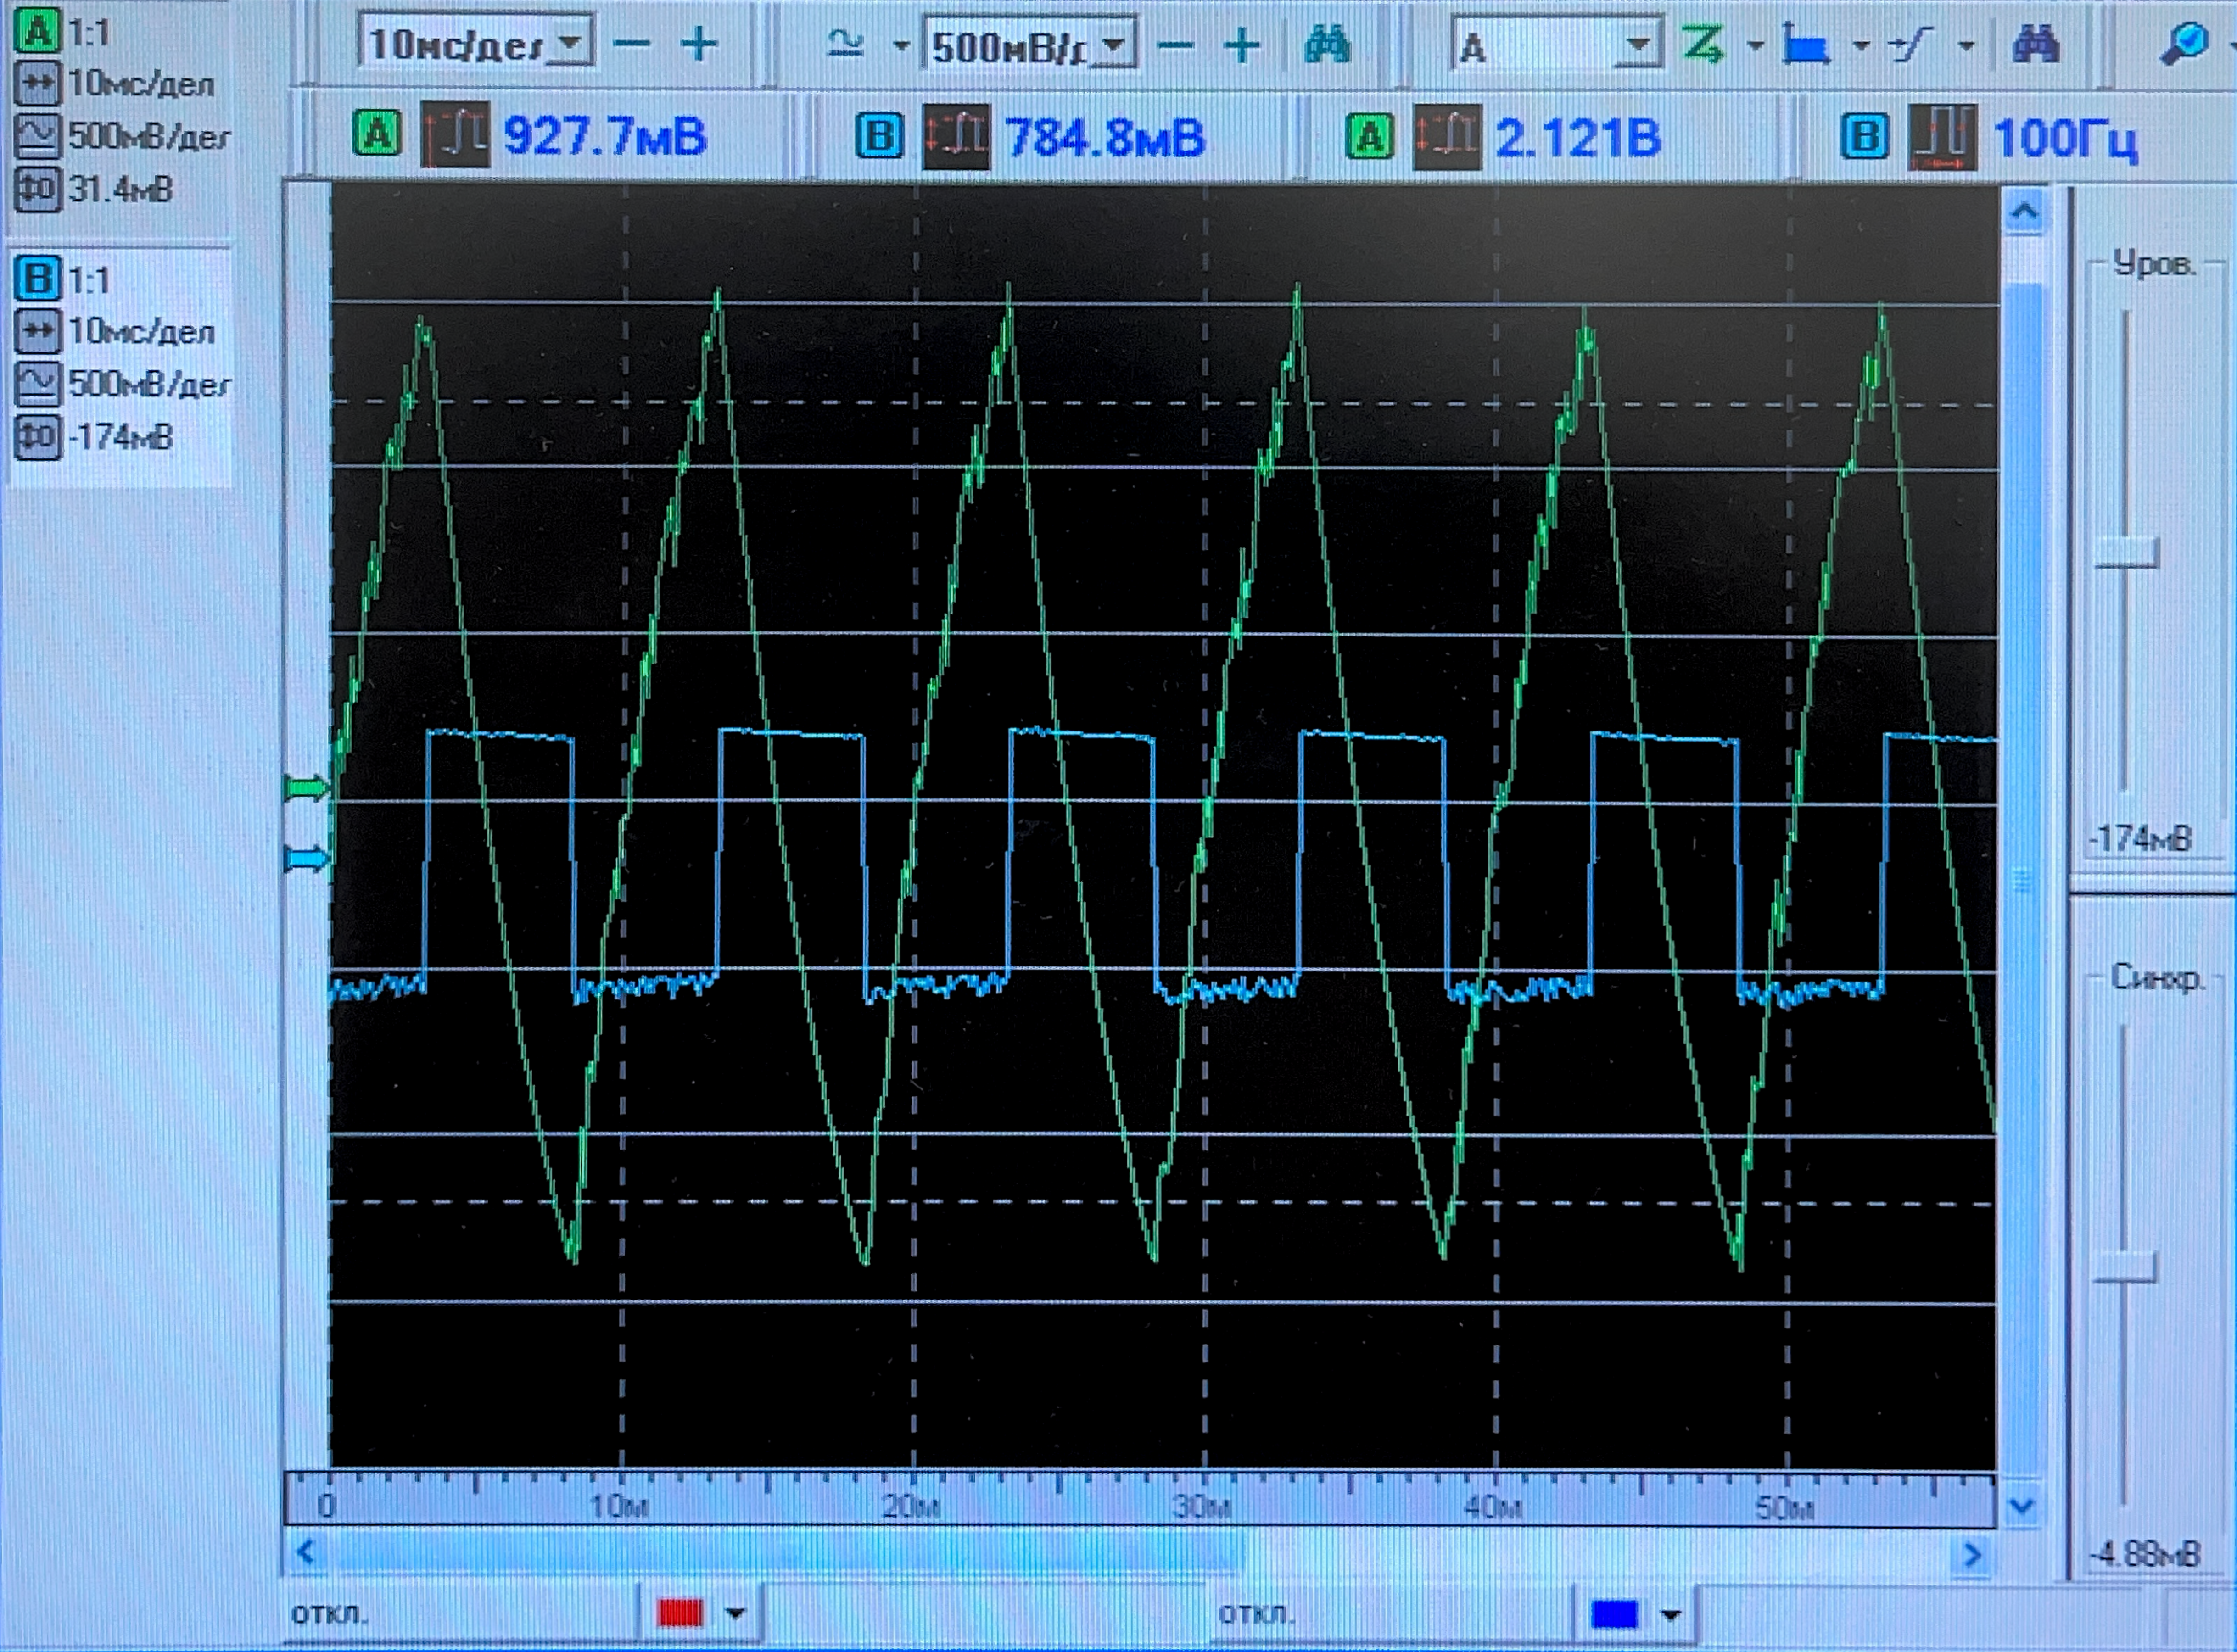
\includegraphics[width=0.7\textwidth]{pictures/osc_rectangle.pdf}
    \caption{Осциллограмма для прямоугольного сигнала на входе интегратора}
    \label{pic:osc_rectangle}
\end{figure}

\clearpage

\subsection*{Триггер Шмитта}

\begin{figure}[h]
    \centering
    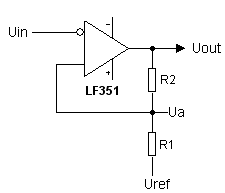
\includegraphics[width=0.35\textwidth]{pictures/ustan-14.png}
    \caption{Схема триггера Шмитта}
    \label{pic:ustan-14}
\end{figure}

\begin{enumerate}
    \item Приняв $U_\textit{ref} = 0$, задав пороги срабатывания $U_{p1} = -0.1$ В, $U_{p2} = 0.1$ В, рассчитаем необходимые параметры схемы:
\end{enumerate}

\begin{equation*}
    \beta = \cfrac{U_{p2}}{U_\textit{max}} = \cfrac{1}{100} = \cfrac{R_1}{R_1 + R_2} \quad \implies \quad R_2 = 99 R_1
\end{equation*}

Параметры установки представлены в таблице \ref{tab:params-14}

\begin{table}[!h]
    \centering
    \caption{Измеренные параметры установки в схеме на рис. \ref{pic:ustan-14}}
    \label{tab:params-14}
    \begin{tabular}{|l|l|l|l|}
        \hline
        $R_1$, Ом & $R_2$, кОм \\ \hline
        665       & 67.12      \\ \hline
    \end{tabular}
\end{table}

\begin{enumerate}[resume]
    \item Подадим на вход колебания с частотой $f = 100$ Гц и амплитудой $A = 2$ В. Зарисуем осциллограмму и изобразим ее на рис. \ref{pic:osc_trigger_0}.
\end{enumerate}


\begin{figure}[!h]
    \centering
    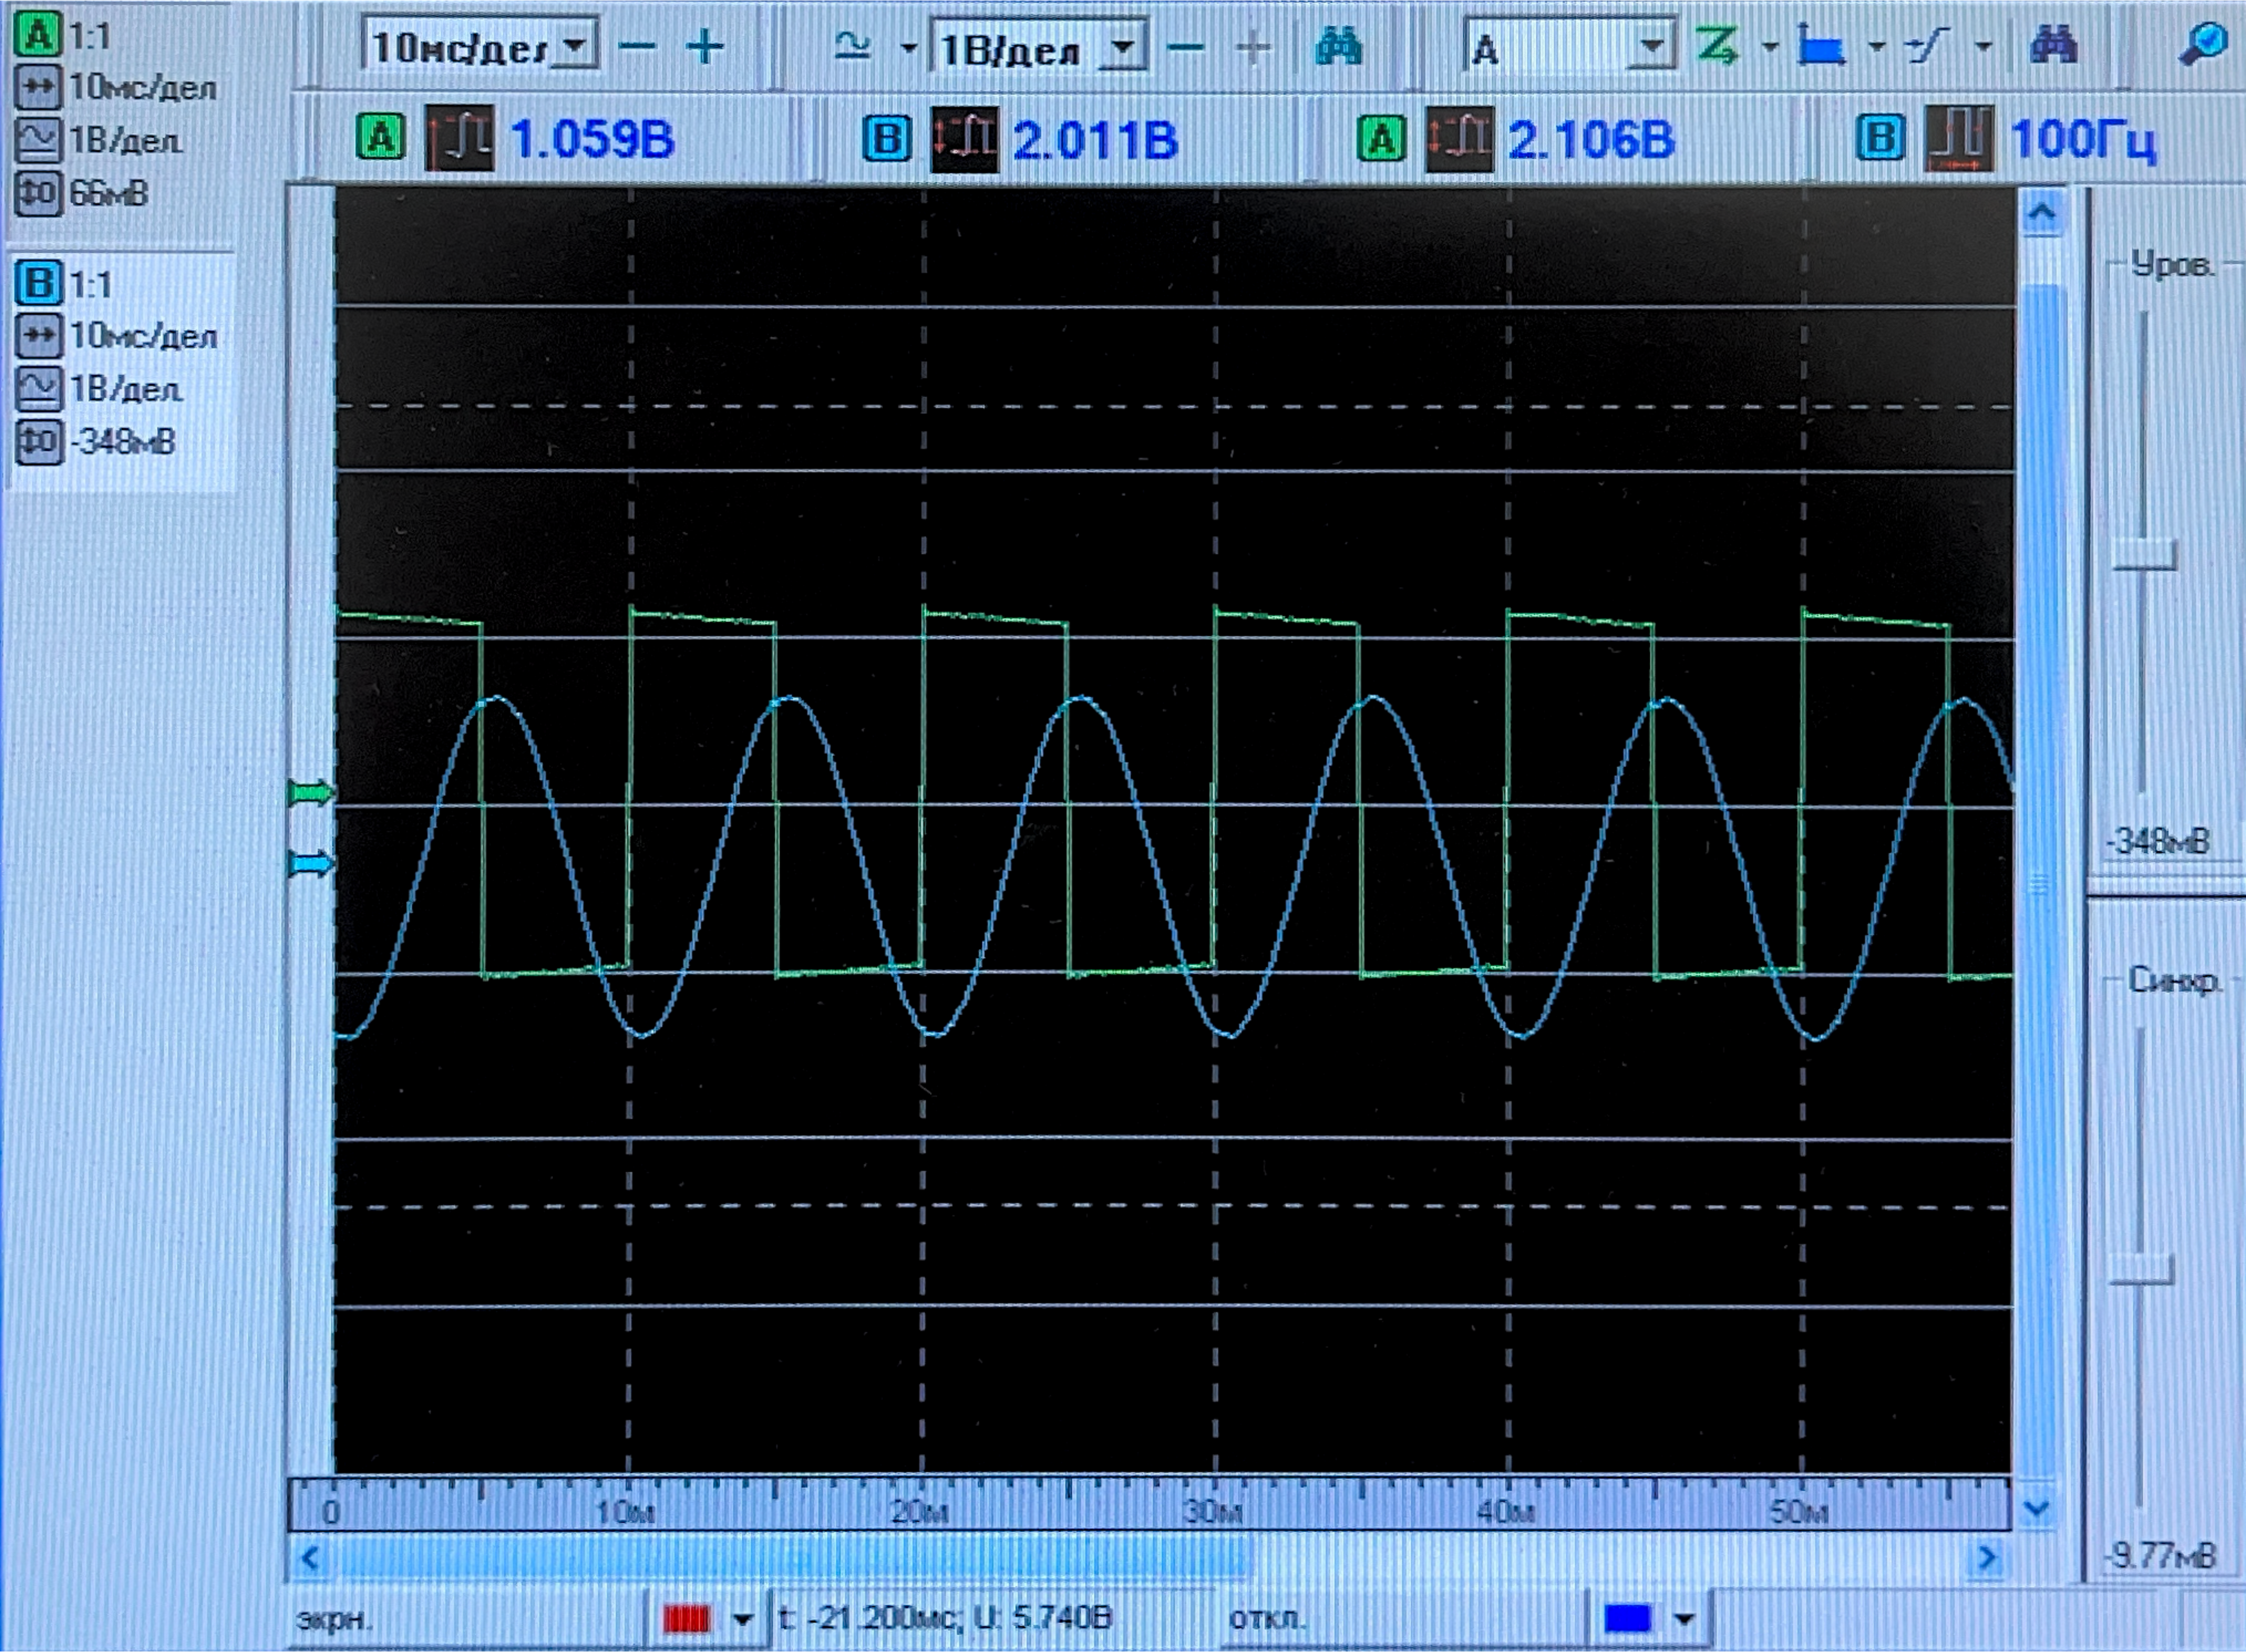
\includegraphics[width=0.7\textwidth]{pictures/osc_trigger_0.pdf}
    \caption{Осциллограмма при $U_{ref} = 0$, $A = 2$ В}
    \label{pic:osc_trigger_0}
\end{figure}
\FloatBarrier

\begin{enumerate}[resume]
    \item Выберем в качестве $U_{ref}$ ненулевое напряжение, повторим предыдущие измерения.
\end{enumerate}
\FloatBarrier

\begin{figure}[!h]
    \centering
    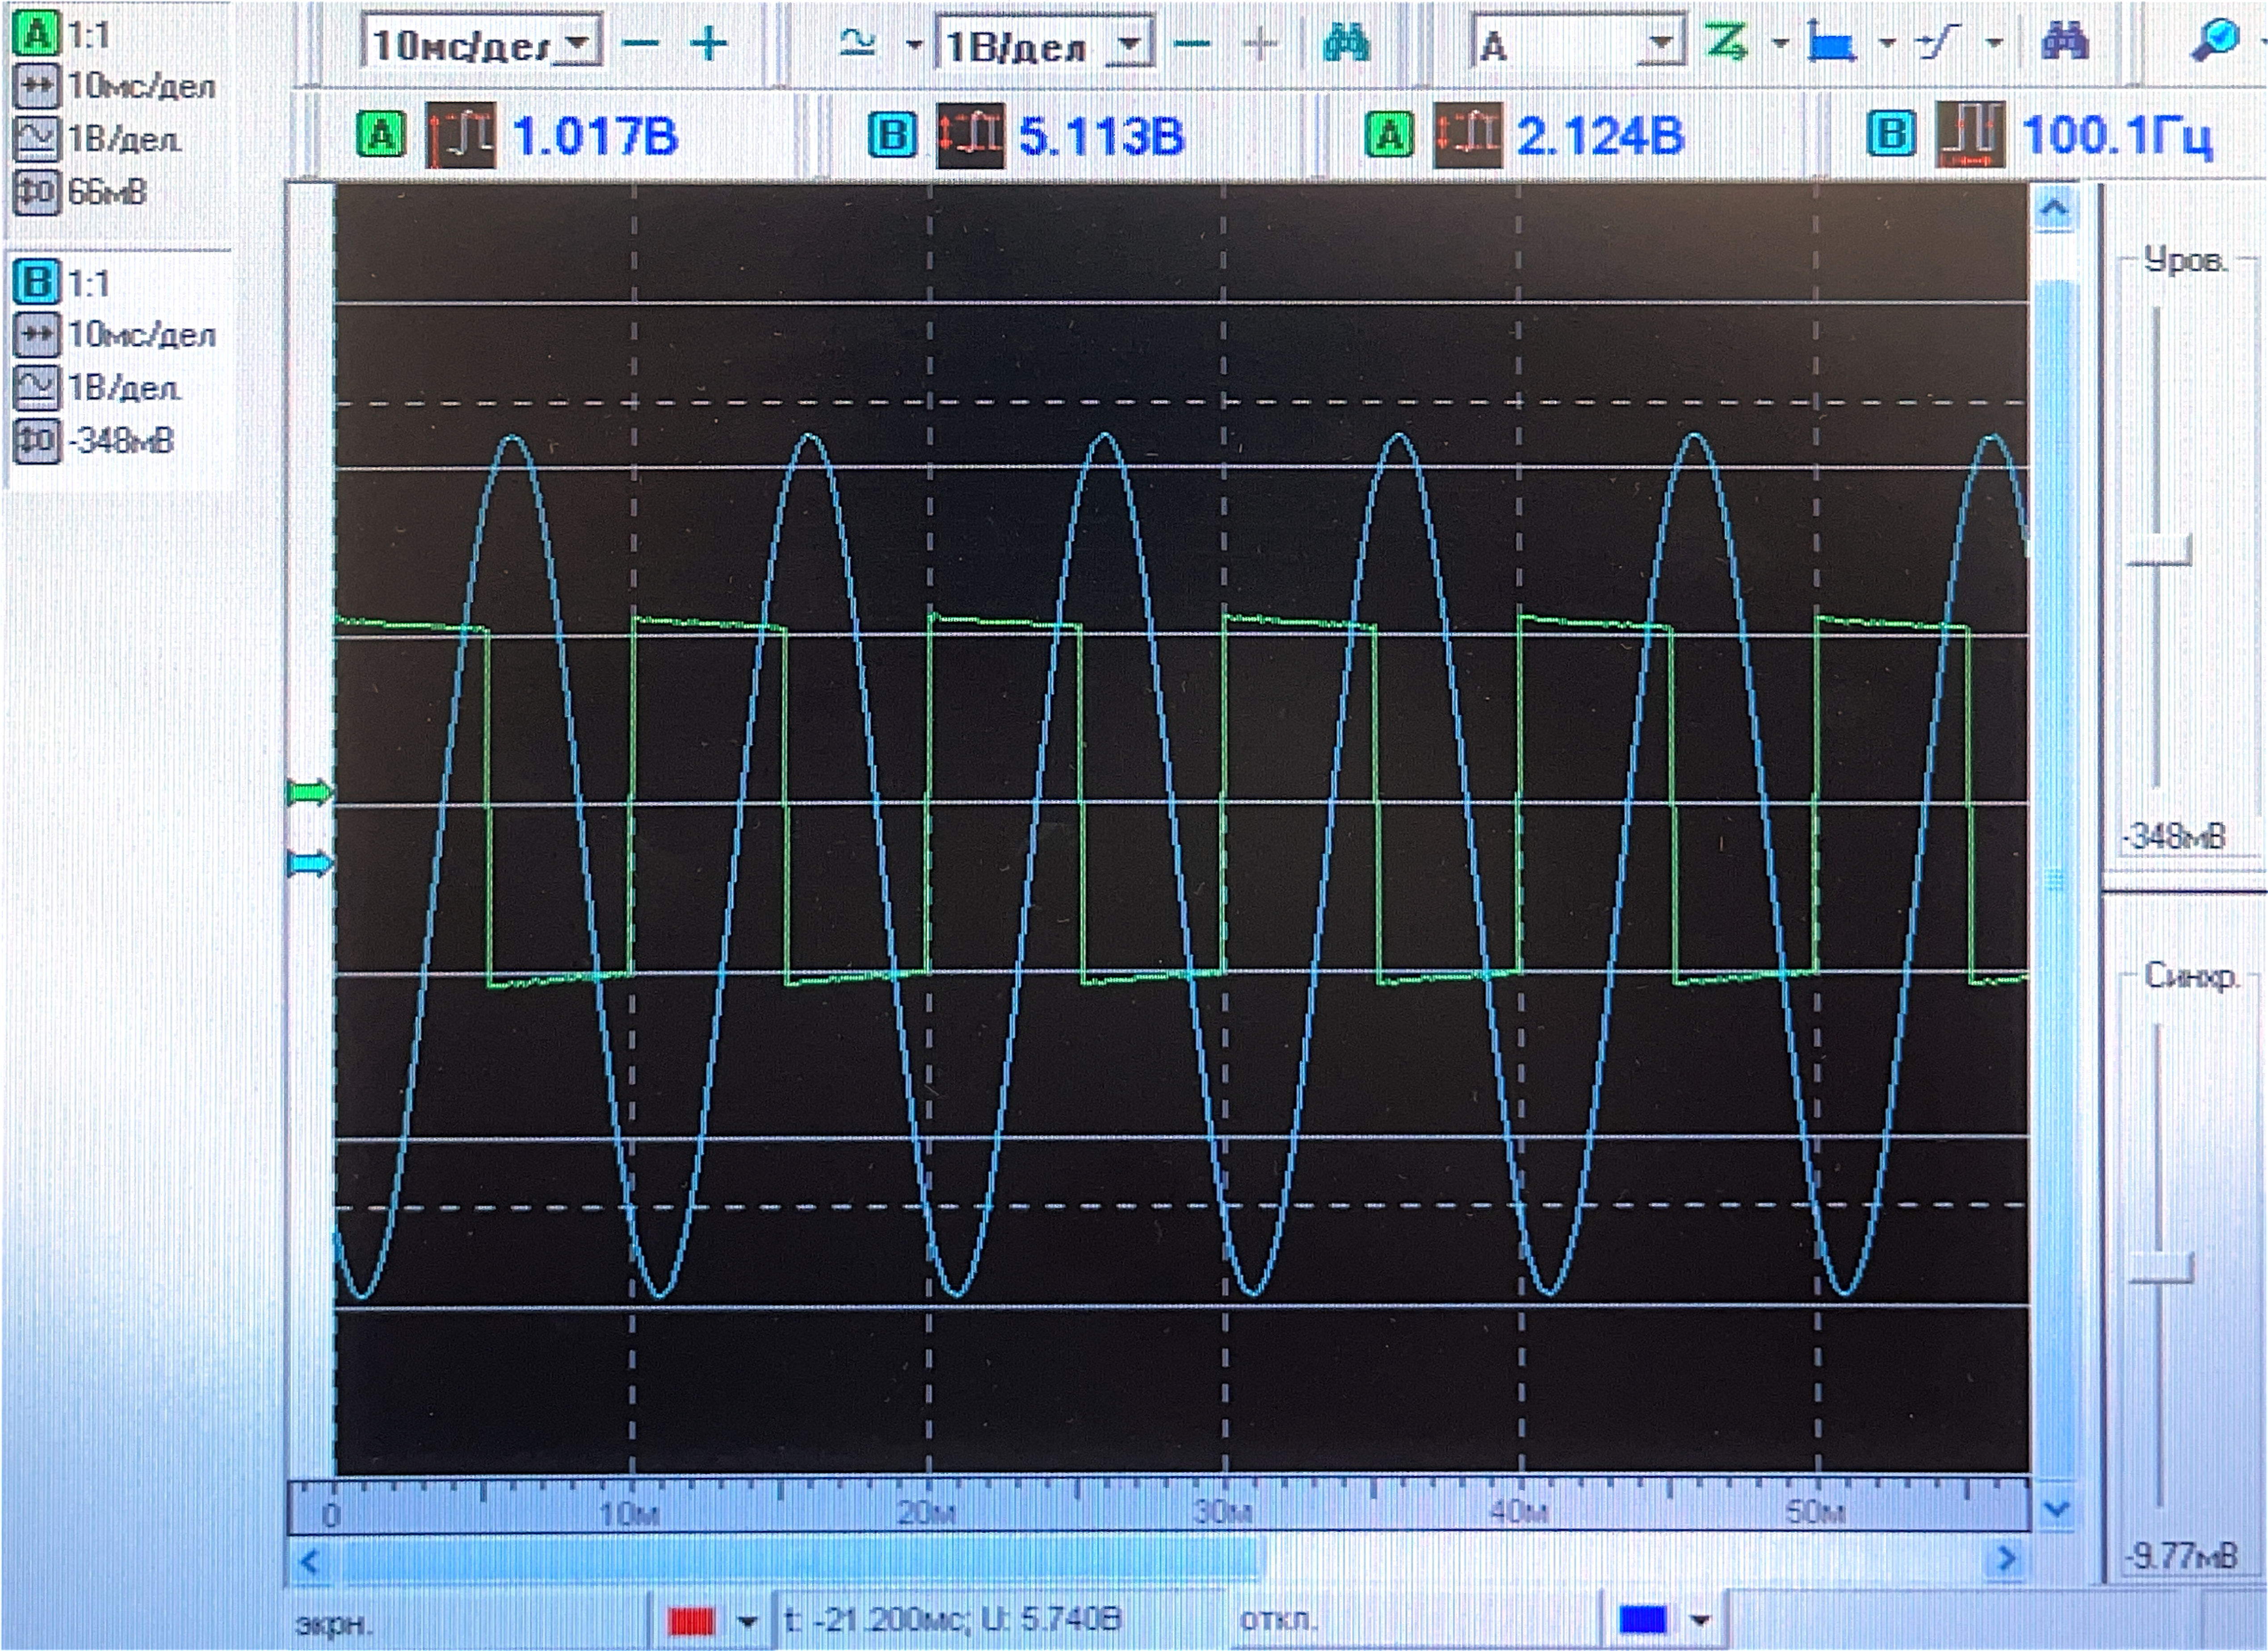
\includegraphics[width=0.7\textwidth]{pictures/osc_trigger_0-115.pdf}
    \caption{Осциллограмма при $U_{ref} = 0.115$ В, $A = 5$ В}
    \label{pic:osc_trigger_0-115}
\end{figure}

\begin{figure}[!h]
    \centering
    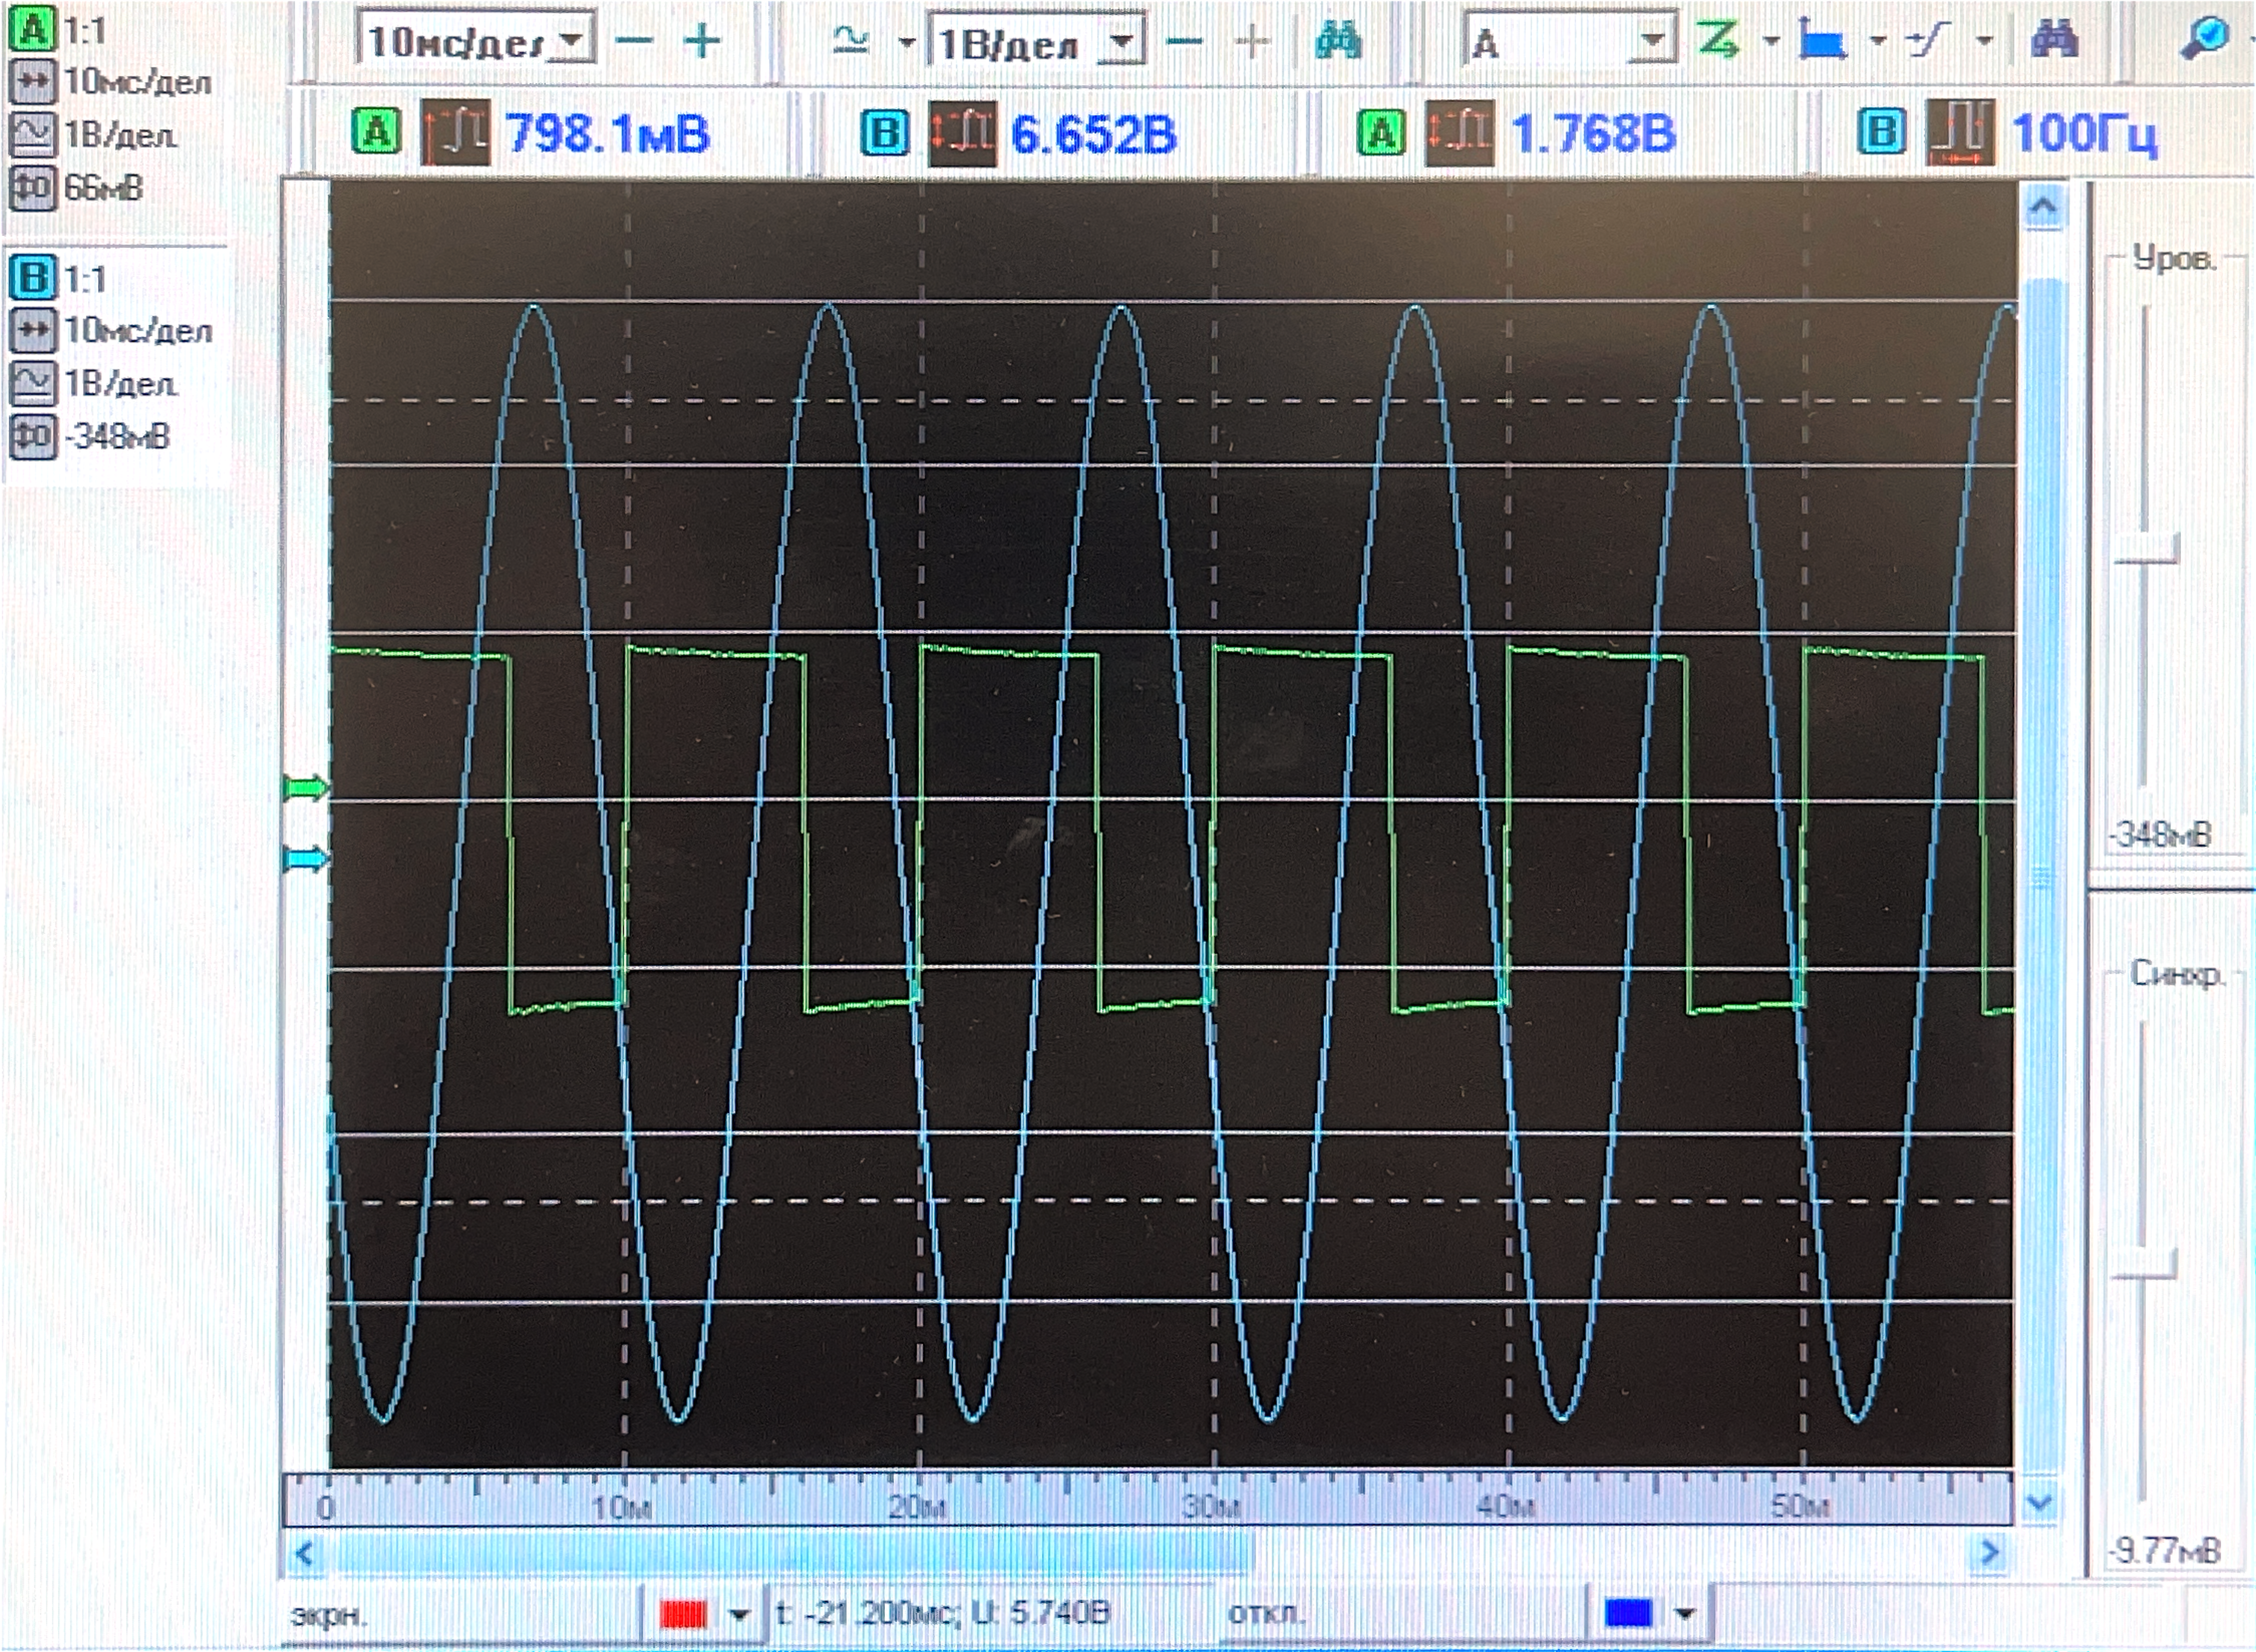
\includegraphics[width=0.7\textwidth]{pictures/osc_trigger_1-06.pdf}
    \caption{Осциллограмма при $U_{ref} = 1.06$ В, $A = 6.5$ В}
    \label{pic:osc_trigger_1-06}
\end{figure}

\FloatBarrier

\subsection*{Самовозбуждающийся мультивибратор}

\FloatBarrier
\begin{figure}[h]
    \centering
    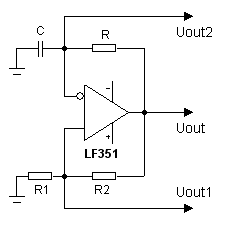
\includegraphics[width=0.35\textwidth]{pictures/ustan-15.png}
    \caption{Схема самовозбуждающегося мультивибратора}
    \label{pic:ustan-15}
\end{figure}


\begin{enumerate}
    \item Рассчитаем элементы схемы мультивибратора, задав $\beta = 0.01$, $T_0 = 0.75$ мс.
\end{enumerate}

\begin{equation*}
    T_0 = 2RC \ln {\left( \cfrac{1 + \beta}{1 - \beta} \right)} = 2RC \ln {\left( 1 + \cfrac{2R_1}{R_2} \right)} 
\end{equation*}

Если взять сопротивления $R_1$ и $R_2$ как в прошлом пункте, то получим из соотношения выше, что

\begin{equation*}
    RC \approx 20 ~ \text{мс}
\end{equation*}

Если взять конденсатор с $C = 1.05$ мкФ, то $R \approx 19$ кОм. Используемые компоненты представлены в таблице \ref{tab:params-15}.


\begin{table}[!h]
    \centering
    \caption{Измеренные параметры установки в схеме на рис. \ref{pic:ustan-15}}
    \label{tab:params-15}
    \begin{tabular}{|l|l|l|l|}
        \hline
        $R_1$, Ом & $R_2$, кОм & $R$, кОм & $C$, мкФ \\ \hline
        665       & 67.12      & 19.85    & 1.05 \\ \hline
    \end{tabular}
\end{table}

\begin{enumerate}[resume]
    \item Соберем схему мультивибратора и зарисуем осциллограммы на выходах $U_{out}$, $U_{out1}$, $U_{out2}$ и изобразим их соответственно на рис. \ref{pic:osc_vibrator_U_out}, \ref{pic:osc_vibrator_U_out1}, \ref{pic:osc_vibrator_U_out2}. Измерения проведены в режиме 1:10.
\end{enumerate}

\begin{figure}[!h]
    \centering
    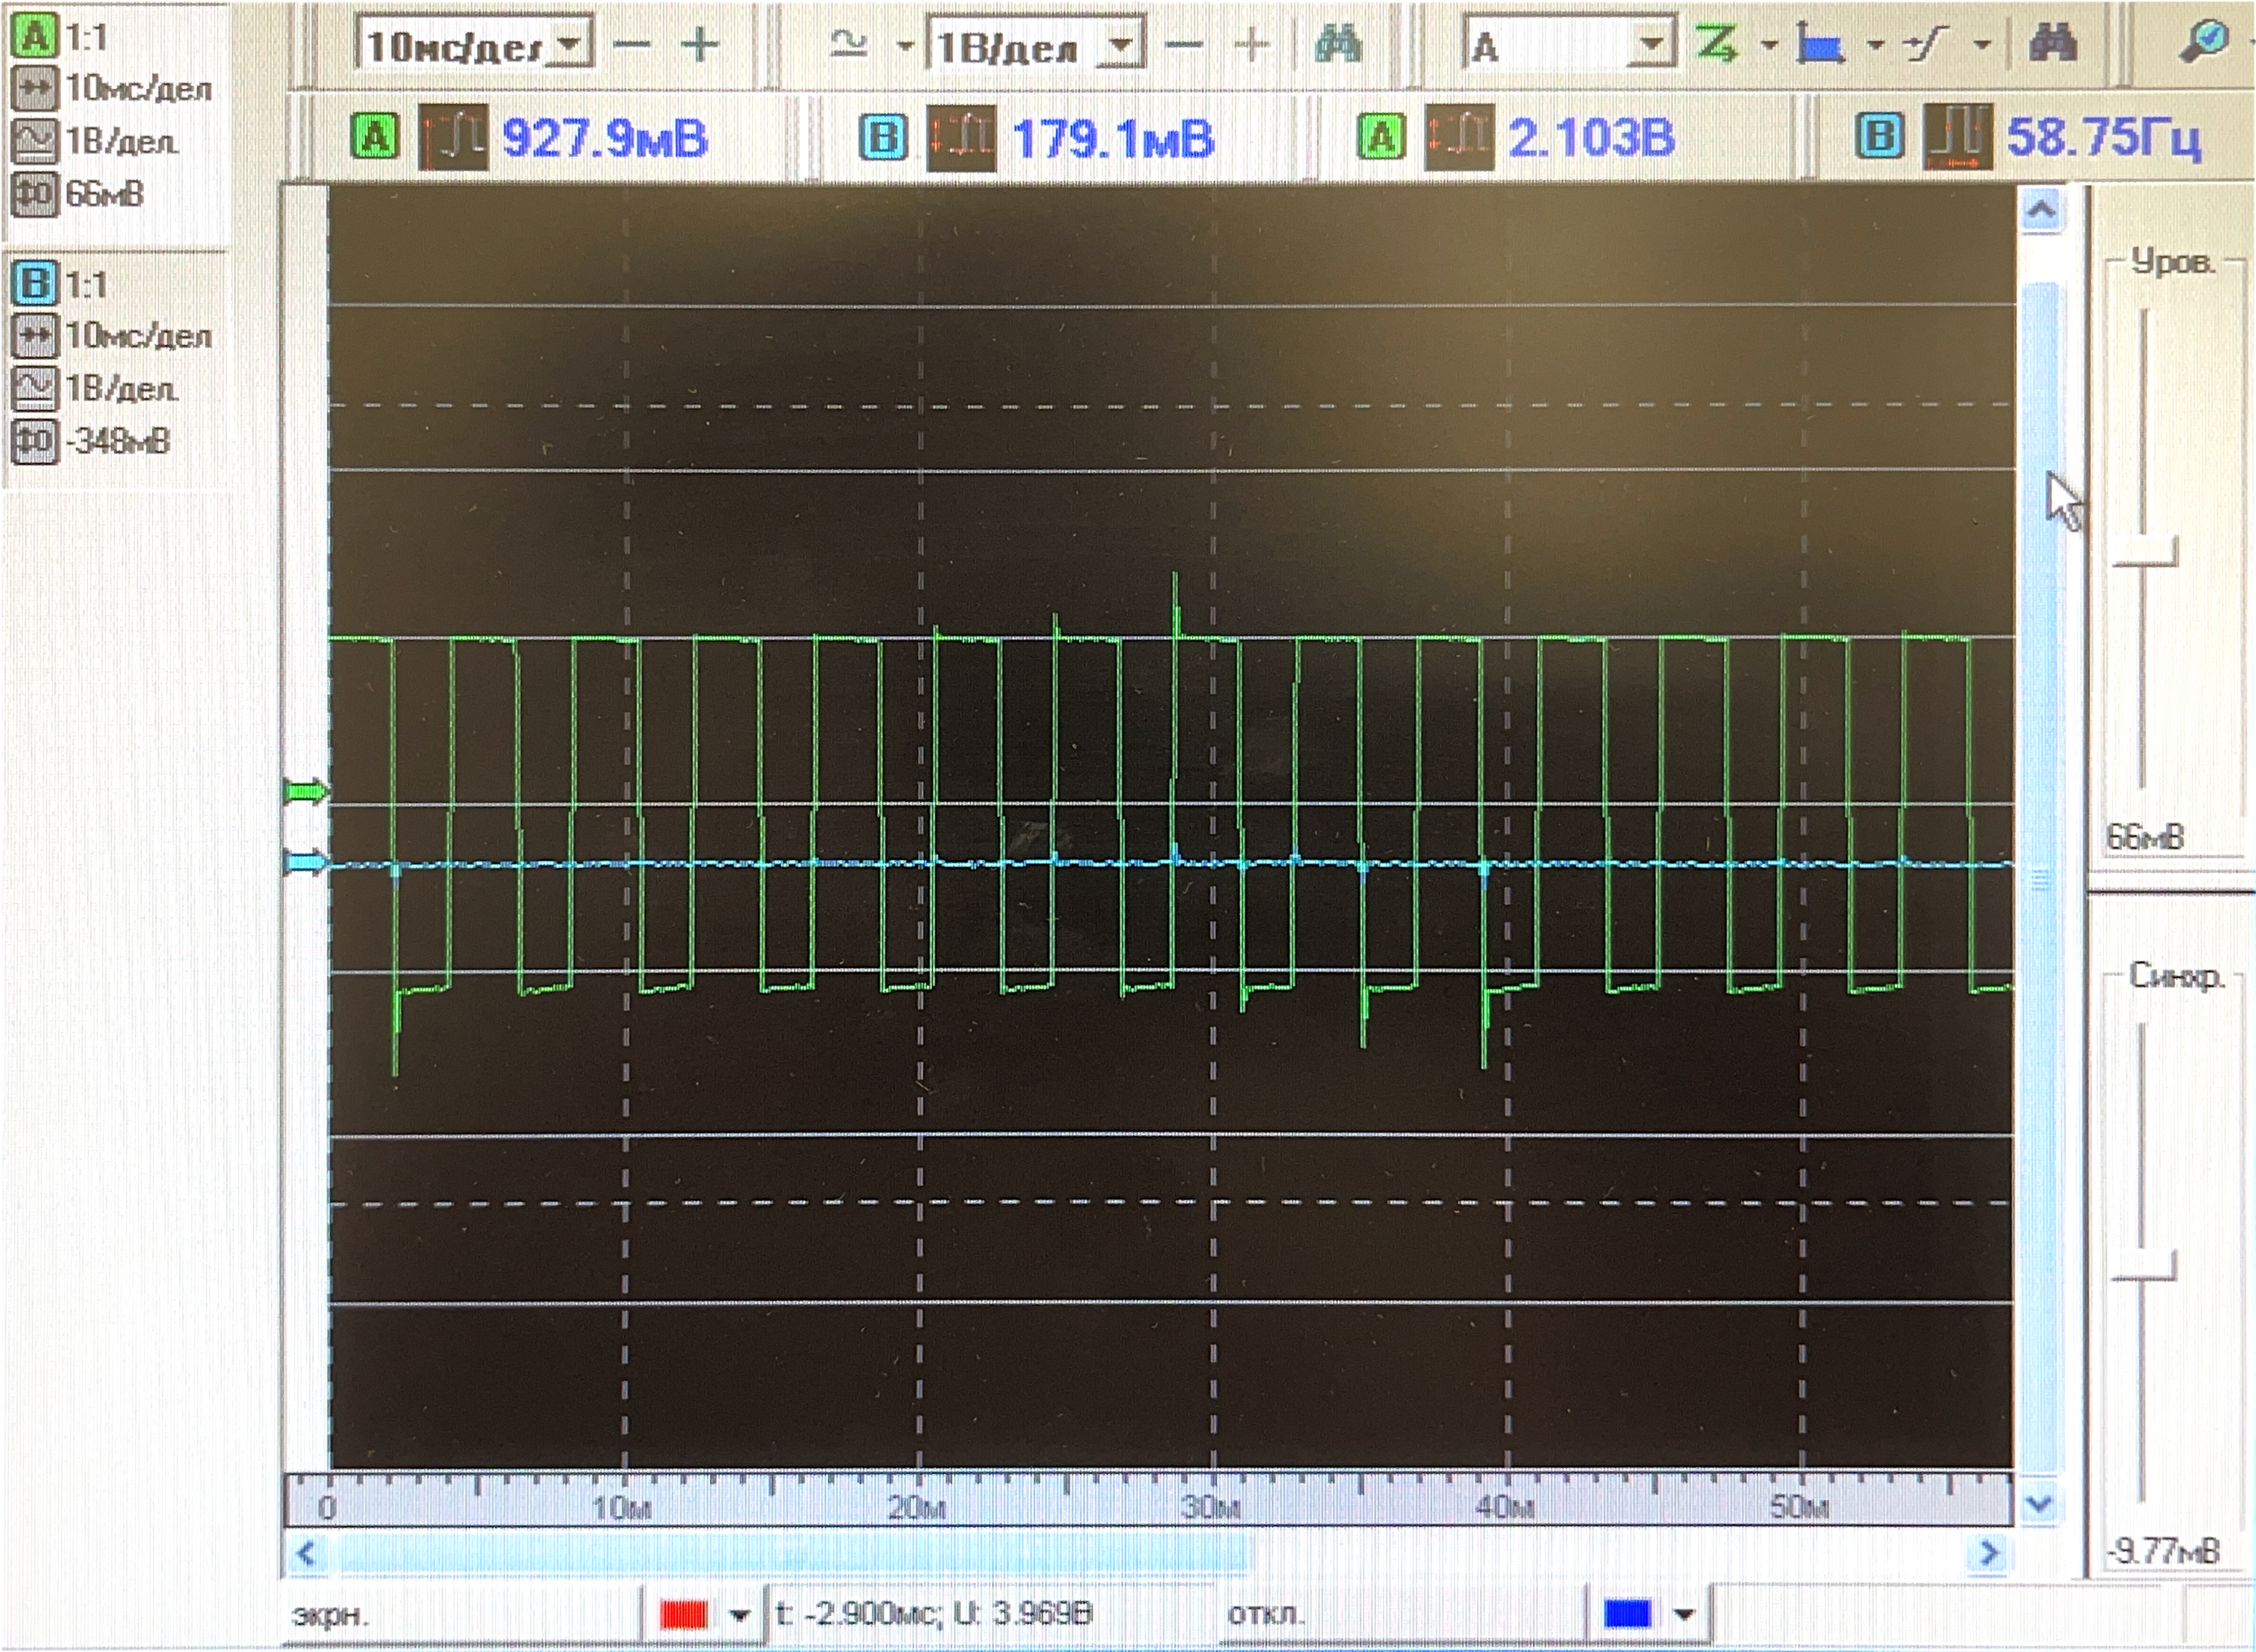
\includegraphics[width=0.7\textwidth]{pictures/osc_vibrator_U_out.pdf}
    \caption{Осциллограмма для сигнала $U_{out}$}
    \label{pic:osc_vibrator_U_out}
\end{figure}
\begin{figure}[!h]
    \centering
    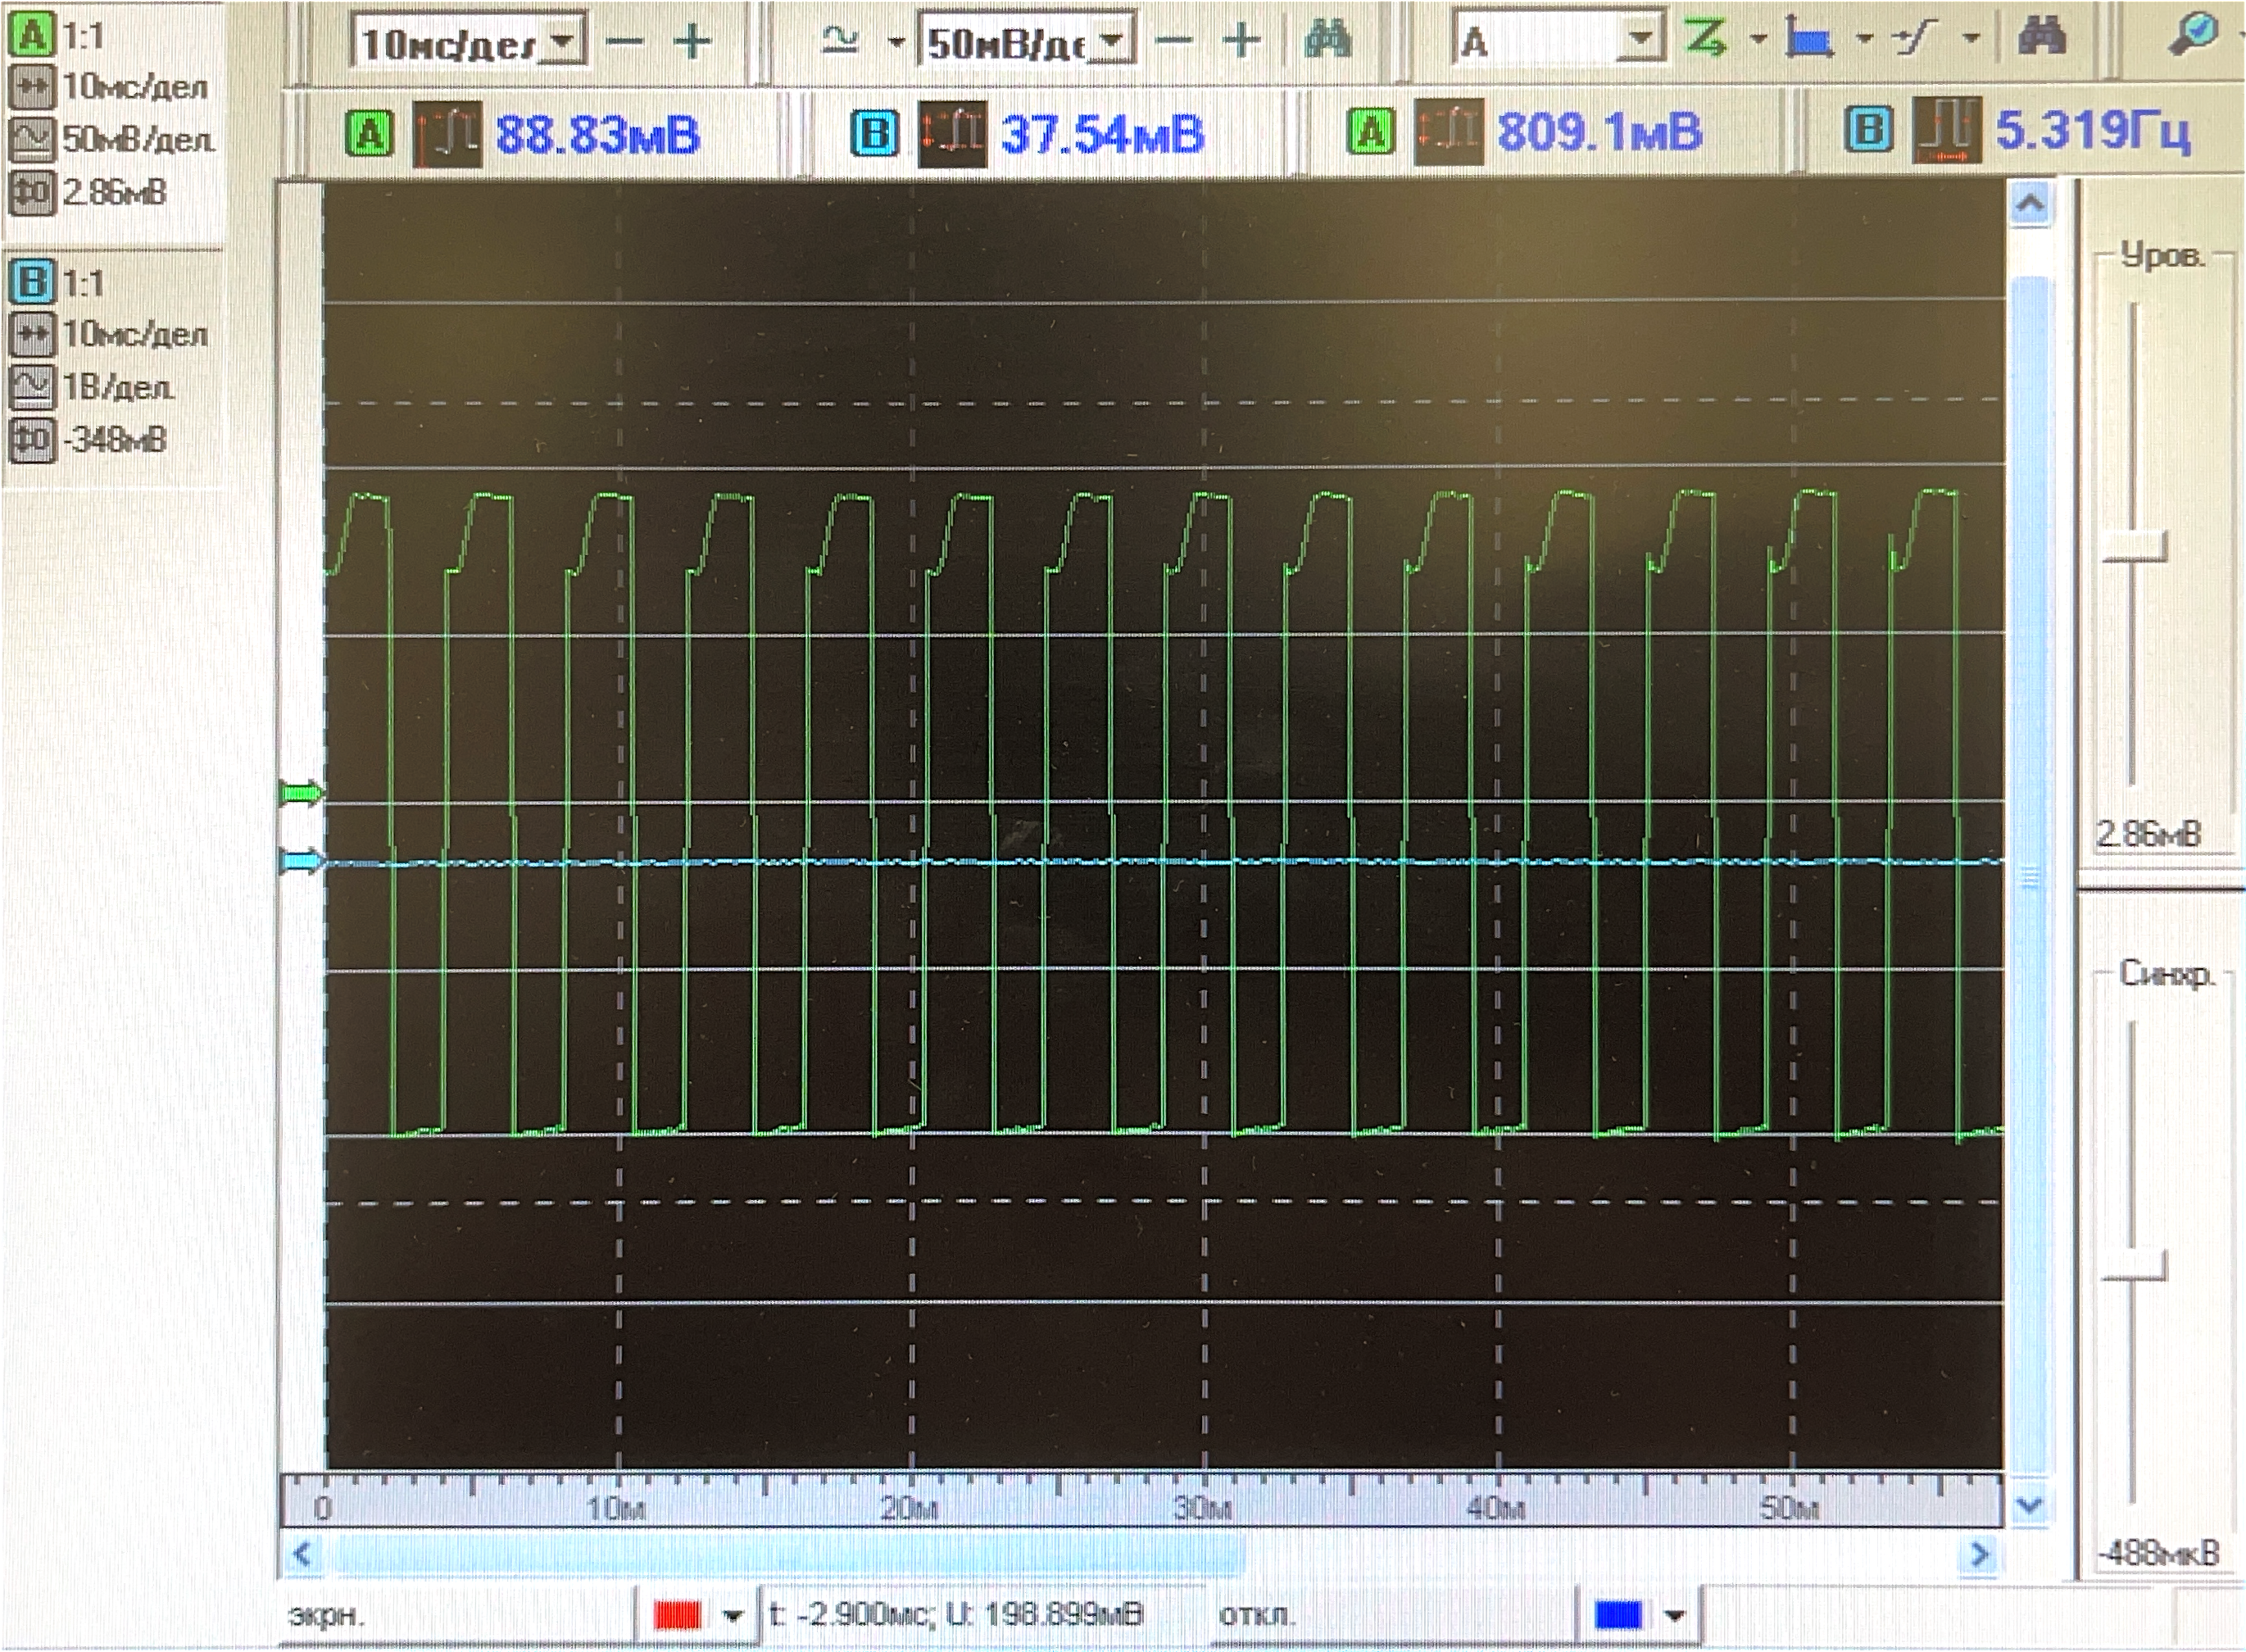
\includegraphics[width=0.7\textwidth]{pictures/osc_vibrator_U_out1.pdf}
    \caption{Осциллограмма для сигнала $U_{out1}$}
    \label{pic:osc_vibrator_U_out1}
\end{figure}
\begin{figure}[!h]
    \centering
    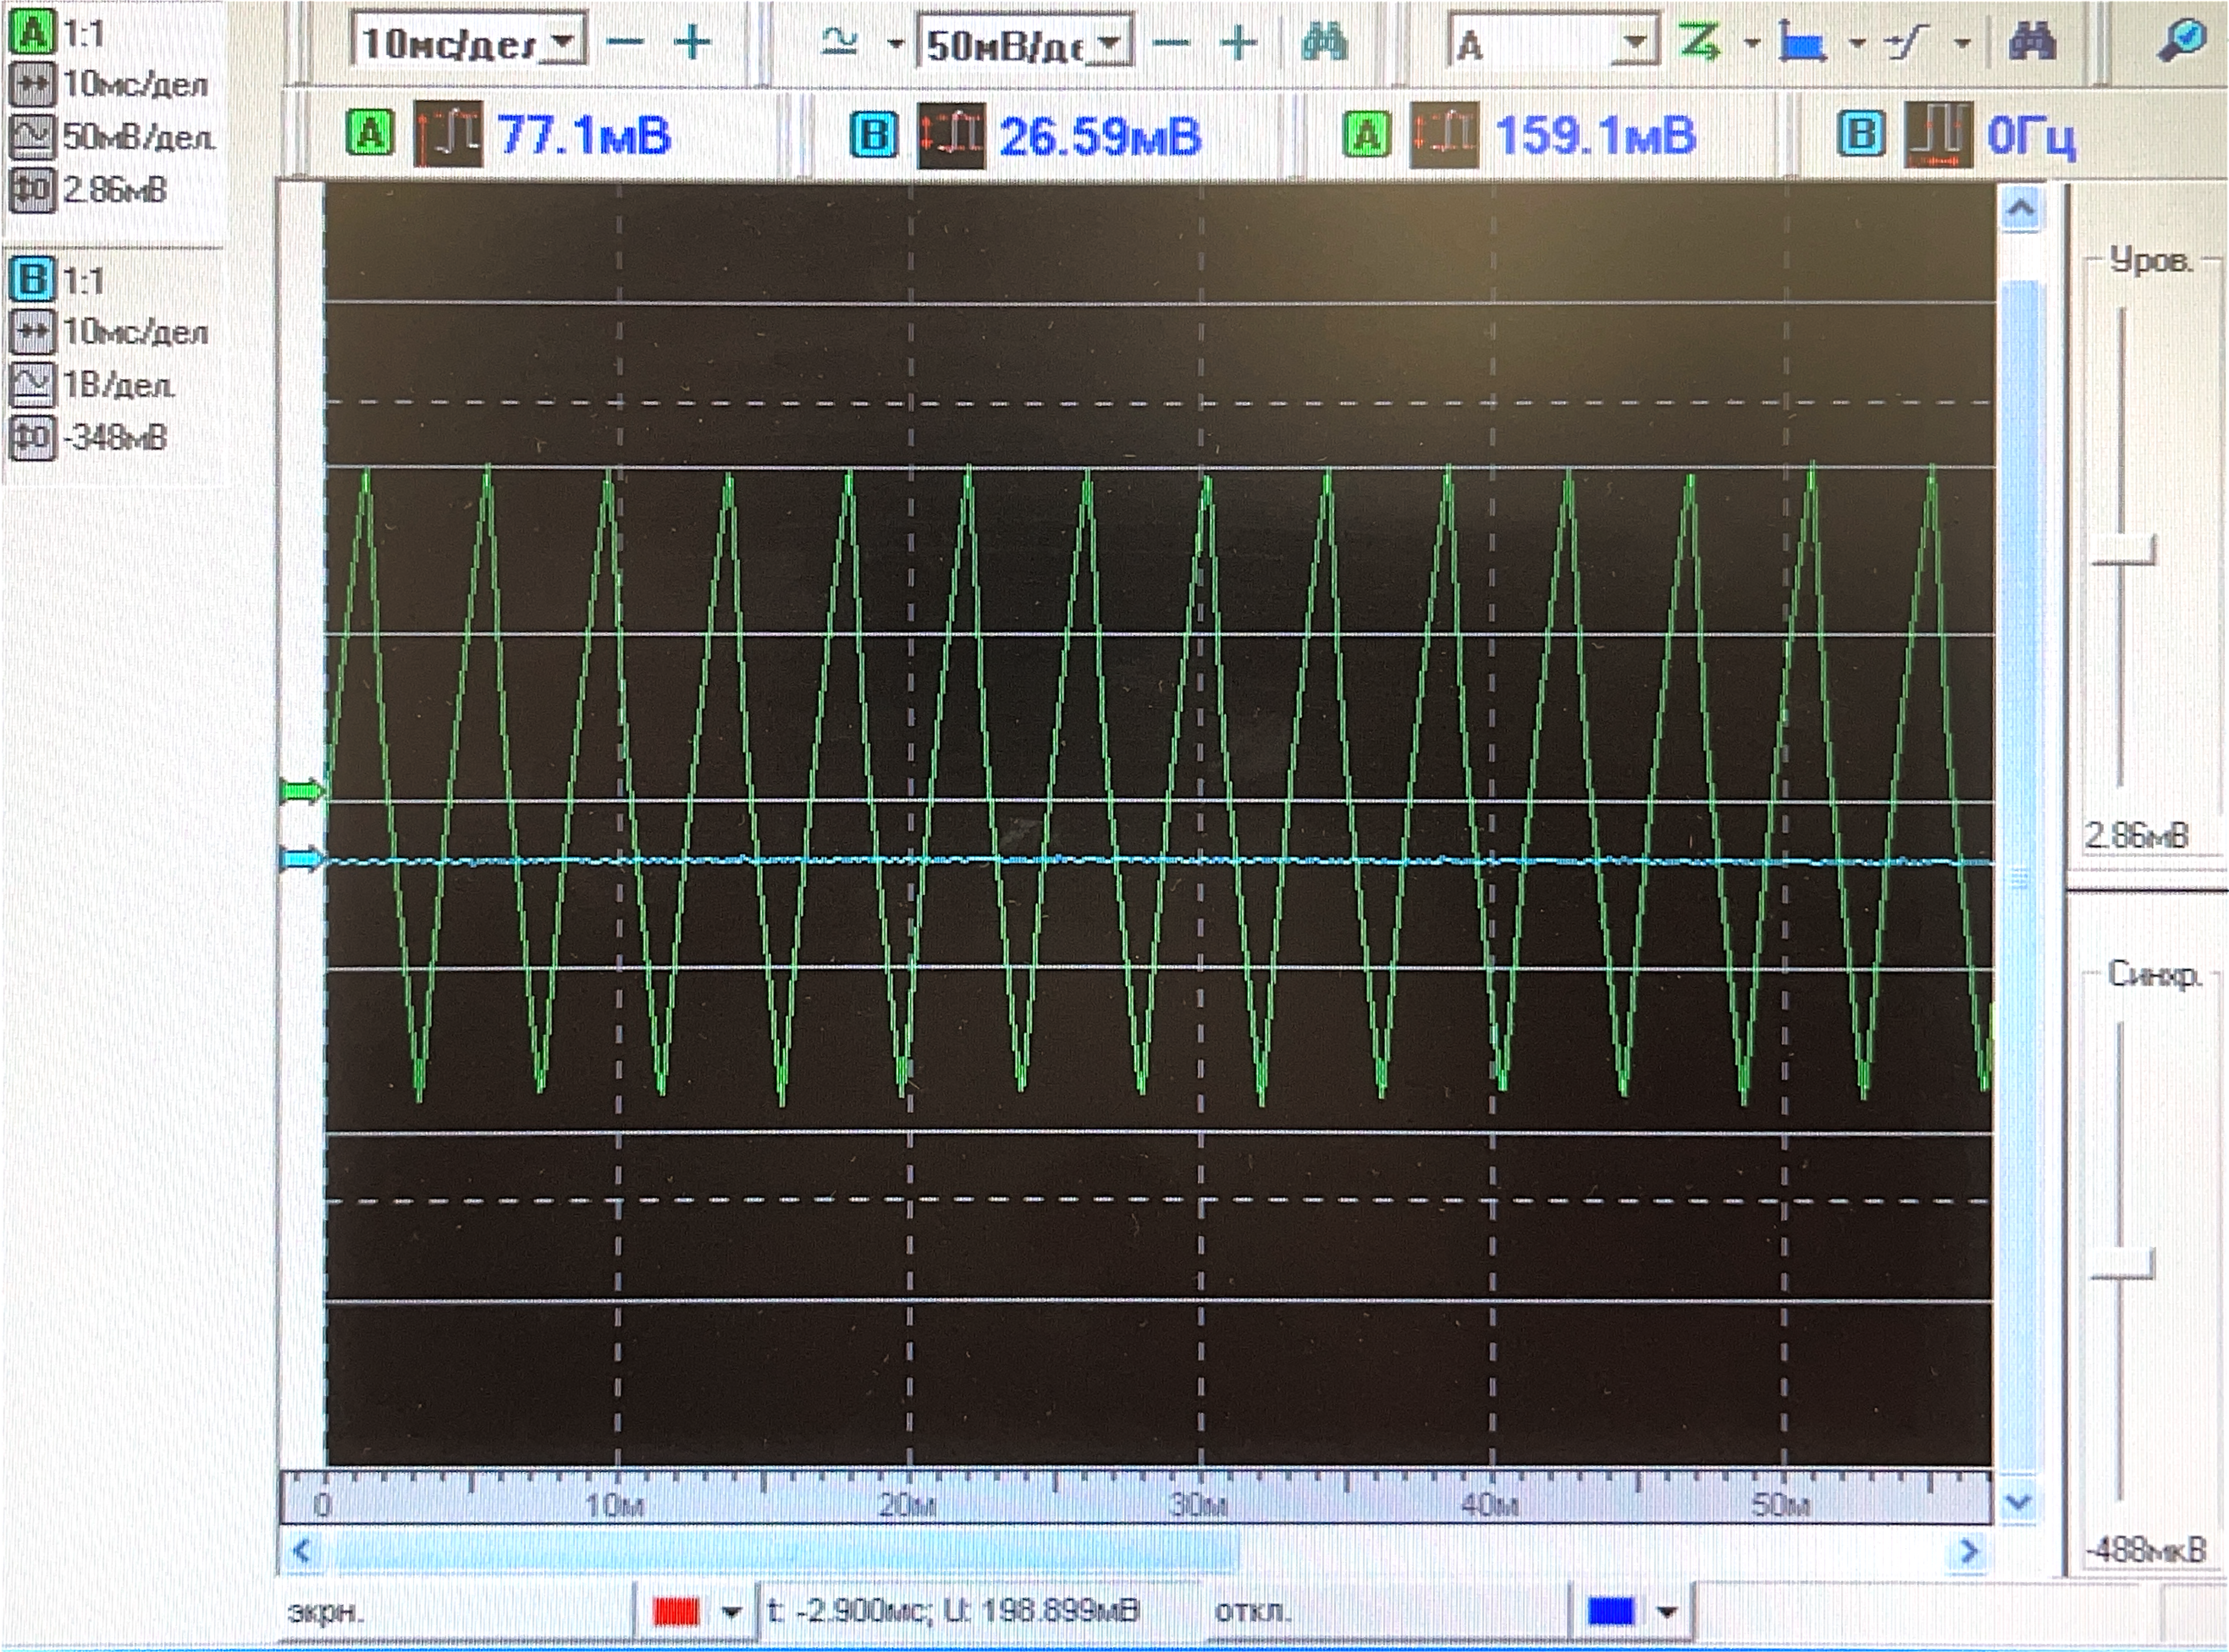
\includegraphics[width=0.7\textwidth]{pictures/osc_vibrator_U_out2.pdf}
    \caption{Осциллограмма для сигнала $U_{out2}$}
    \label{pic:osc_vibrator_U_out2}
\end{figure}

\FloatBarrier

Для каждого выхода измерим амплитудные и временные характеристики и запишем в таблицу \ref{tab:vibrator_characteristics}.


\begin{table}[!h]
    \centering
    \caption{Амплитудные и частотные характеристики сигнала на выходах мультивибратора}
    \label{tab:vibrator_characteristics}
    \begin{tabular}{|l|l|l|l|}
        \hline
        ~          & $U_{out}$ & $U_{out1}$ & $U_{out2}$ \\ \hline
        $A$, В     & 9.279     & 0.883      & 0.771      \\ \hline
        $\tau$, мс & 4.1       & 4          & 4          \\ \hline
    \end{tabular}
\end{table}


\end{document}
